\documentclass[11pt]{article}
\usepackage[textwidth=18.0cm, textheight=23.0cm, top=2.0cm]{geometry}
\usepackage{pst-all}
\usepackage{amssymb}
\usepackage{tikz}
\usepackage{underscore}\begin{document}
\pagestyle{empty}


ClassName: \underline{\textbf{Class_07.2bp-42}}
\par
BinSize: \underline{\textbf{100 × 100}}
\par
ReduceSize: \underline{\textbf{100 × 100}}
\par
TypeNum: \underline{\textbf{99}}
\par
Num: \underline{\textbf{100}}
\par
OutS: \underline{\textbf{250000}}
\par
InS: \underline{\textbf{207677}}
\par
Rate: \underline{\textbf{0.831}}
\par
UB: \underline{\textbf{25}}
\par
LB0: \underline{\textbf{25}}
\par
LB: \underline{\textbf{25}}
\par
LBWithCut: \underline{\textbf{25}}
\par
NodeCut: \underline{\textbf{0}}
\par
ExtendedNodeCnt: \underline{\textbf{1}}
\par
GenNodeCnt: \underline{\textbf{1}}
\par
PrimalNode: \underline{\textbf{0}}
\par
ColumnCount: \underline{\textbf{25}}
\par
TotalCutCount: \underline{\textbf{0}}
\par
RootCutCount: \underline{\textbf{0}}
\par
LPSolverCnt: \underline{\textbf{1}}
\par
PricingSolverCnt: \underline{\textbf{0}}
\par
BranchAndBoundNum: \underline{\textbf{1}}
\par
isOpt: \underline{\textbf{true}}
\par
TimeOnInitSolution: \underline{\textbf{120.030 s}}
\par
TimeOnPrimal: \underline{\textbf{0.000 s}}
\par
TimeOnPricing: \underline{\textbf{0.000 s}}
\par
TimeOnRmp: \underline{\textbf{0.093 s}}
\par
TotalTime: \underline{\textbf{120.186 s}}
\par
\newpage


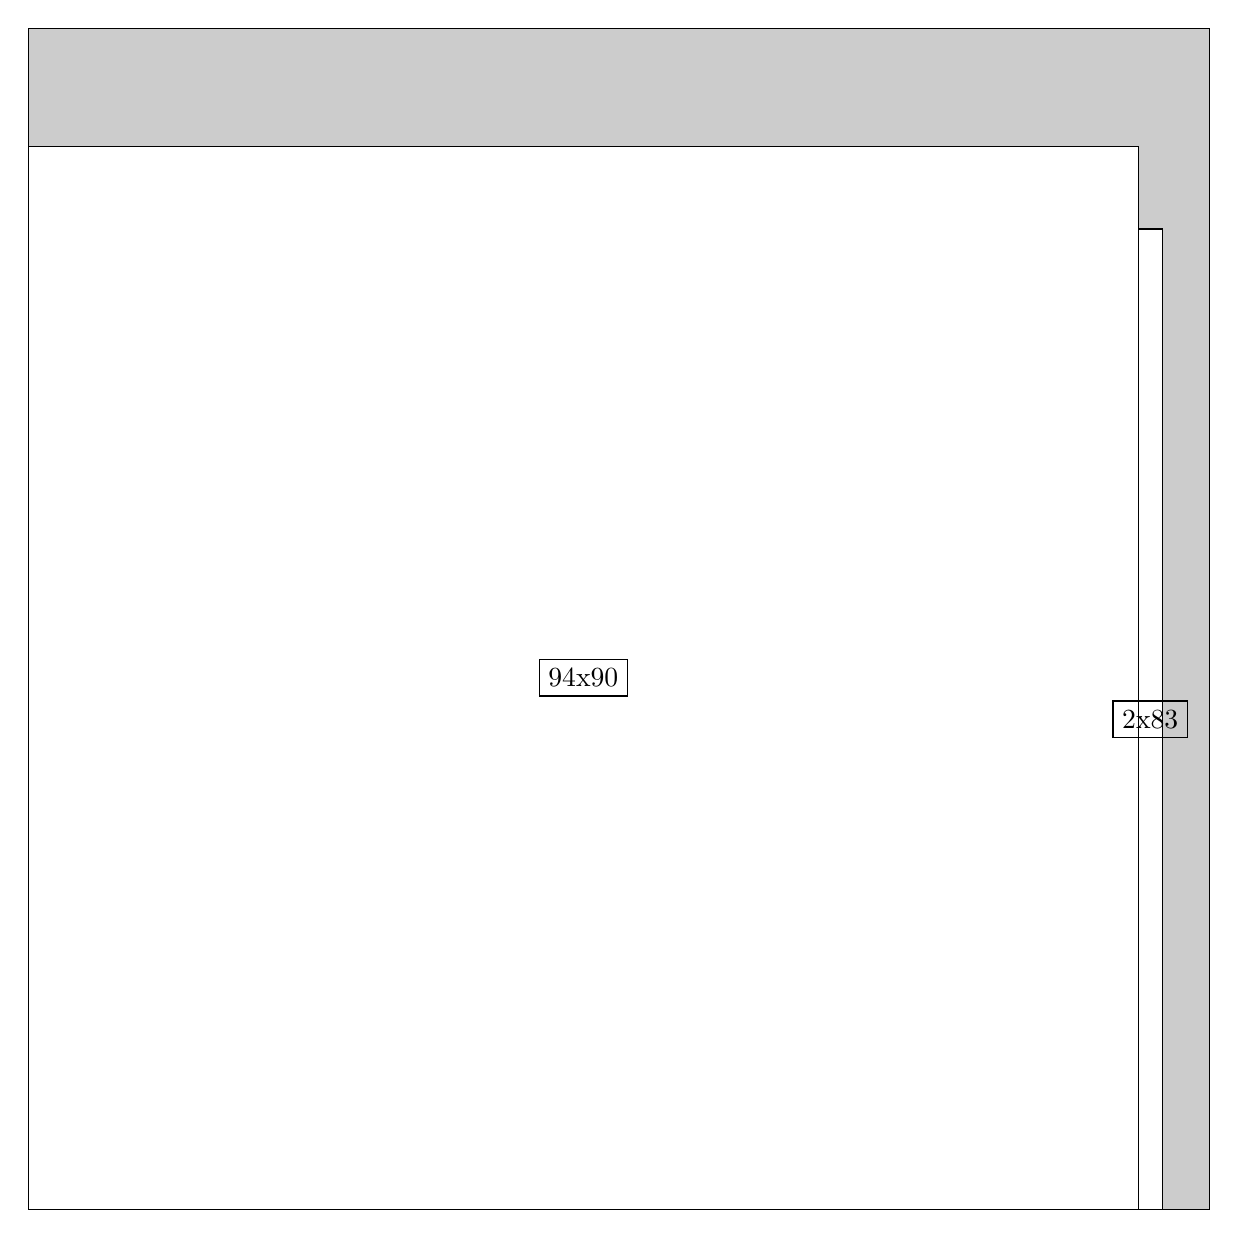
\begin{tikzpicture}[shorten >=1pt,scale=1.0,every node/.style={scale=1.0},->]
\tikzstyle{vertex}=[circle,fill=black!25,minimum size=14pt,inner sep=0pt]
\filldraw[fill=gray!40!white, draw=black] (0,0) rectangle (15.0,15.0);
\foreach \name/\x/\y/\w/\h in {94x90/0.0/0.0/14.1/13.5,2x83/14.1/0.0/0.3/12.45}
\filldraw[fill=white!40!white, draw=black] (\x,\y) rectangle node[draw] (\name) {\name} ++(\w,\h);
\end{tikzpicture}


w =94 , h =90 , x =0 , y =0 , v =8460
\par
w =2 , h =83 , x =94 , y =0 , v =166
\par
\newpage


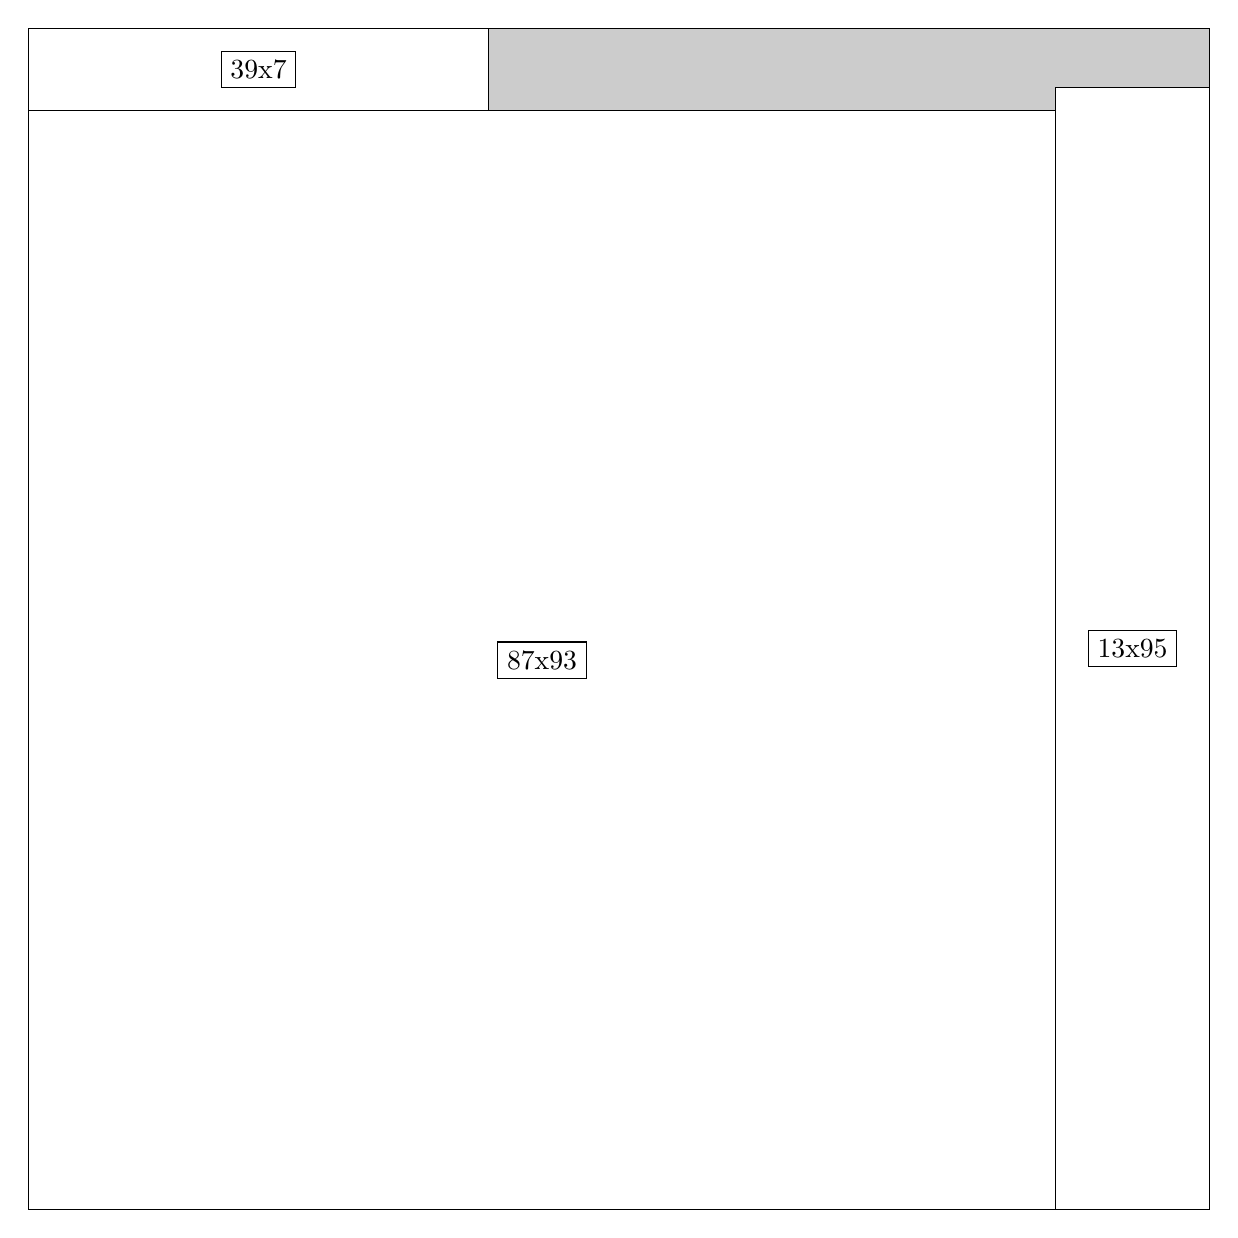
\begin{tikzpicture}[shorten >=1pt,scale=1.0,every node/.style={scale=1.0},->]
\tikzstyle{vertex}=[circle,fill=black!25,minimum size=14pt,inner sep=0pt]
\filldraw[fill=gray!40!white, draw=black] (0,0) rectangle (15.0,15.0);
\foreach \name/\x/\y/\w/\h in {87x93/0.0/0.0/13.049999999999999/13.95,13x95/13.049999999999999/0.0/1.95/14.25,39x7/0.0/13.95/5.85/1.05}
\filldraw[fill=white!40!white, draw=black] (\x,\y) rectangle node[draw] (\name) {\name} ++(\w,\h);
\end{tikzpicture}


w =87 , h =93 , x =0 , y =0 , v =8091
\par
w =13 , h =95 , x =87 , y =0 , v =1235
\par
w =39 , h =7 , x =0 , y =93 , v =273
\par
\newpage


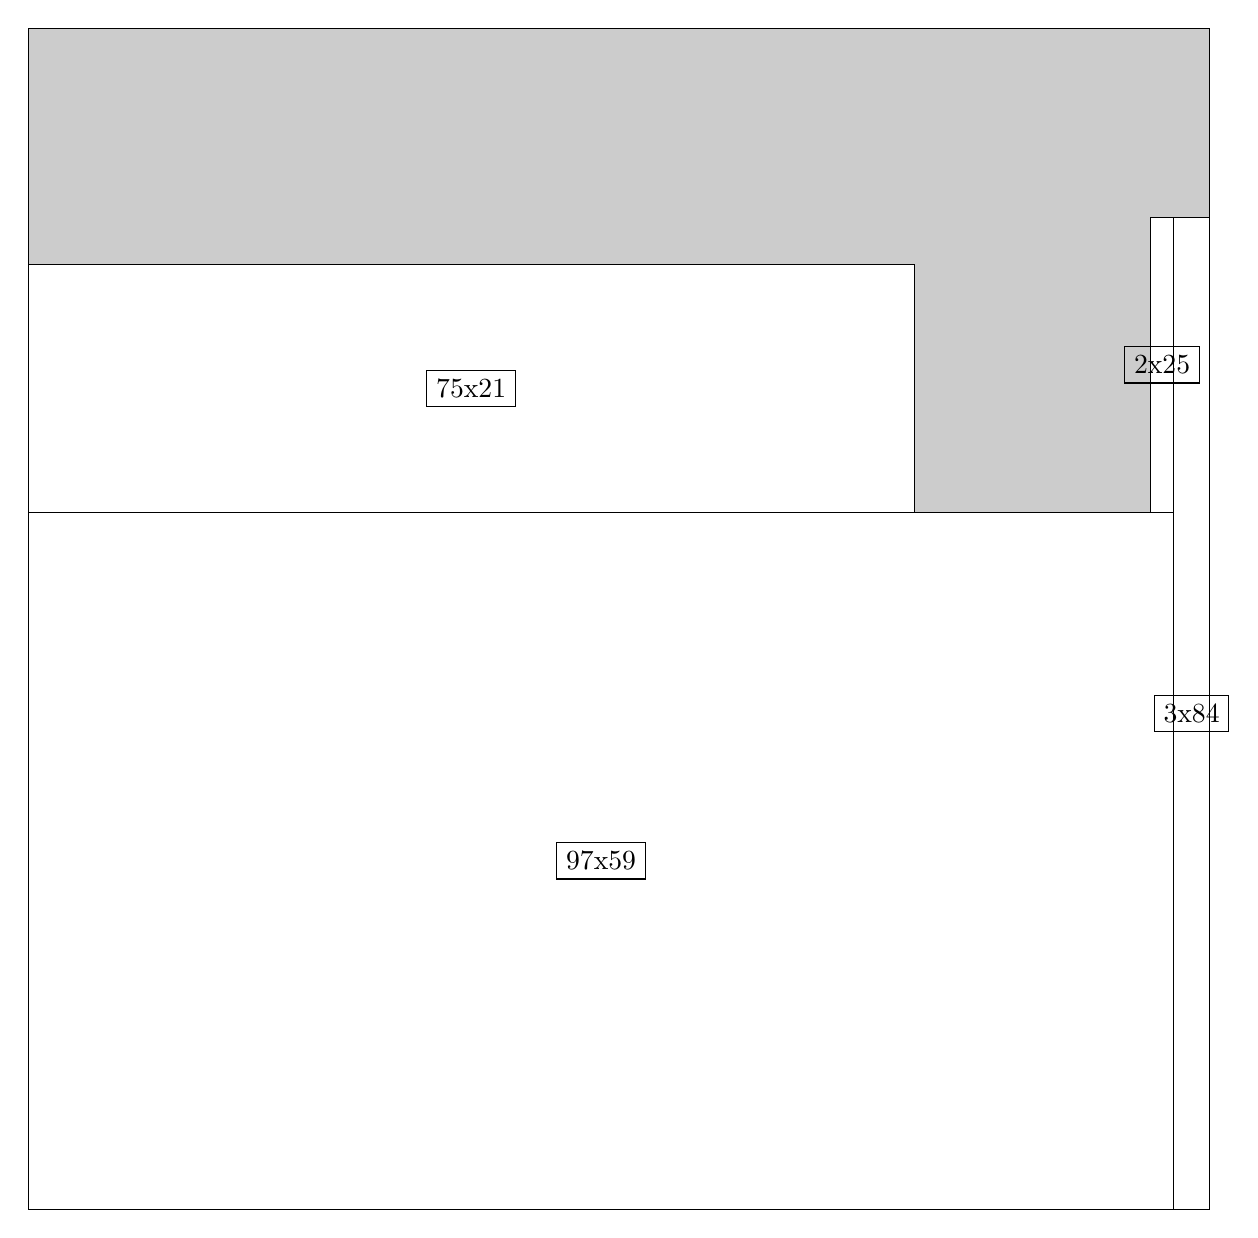
\begin{tikzpicture}[shorten >=1pt,scale=1.0,every node/.style={scale=1.0},->]
\tikzstyle{vertex}=[circle,fill=black!25,minimum size=14pt,inner sep=0pt]
\filldraw[fill=gray!40!white, draw=black] (0,0) rectangle (15.0,15.0);
\foreach \name/\x/\y/\w/\h in {97x59/0.0/0.0/14.549999999999999/8.85,75x21/0.0/8.85/11.25/3.15,3x84/14.549999999999999/0.0/0.44999999999999996/12.6,2x25/14.25/8.85/0.3/3.75}
\filldraw[fill=white!40!white, draw=black] (\x,\y) rectangle node[draw] (\name) {\name} ++(\w,\h);
\end{tikzpicture}


w =97 , h =59 , x =0 , y =0 , v =5723
\par
w =75 , h =21 , x =0 , y =59 , v =1575
\par
w =3 , h =84 , x =97 , y =0 , v =252
\par
w =2 , h =25 , x =95 , y =59 , v =50
\par
\newpage


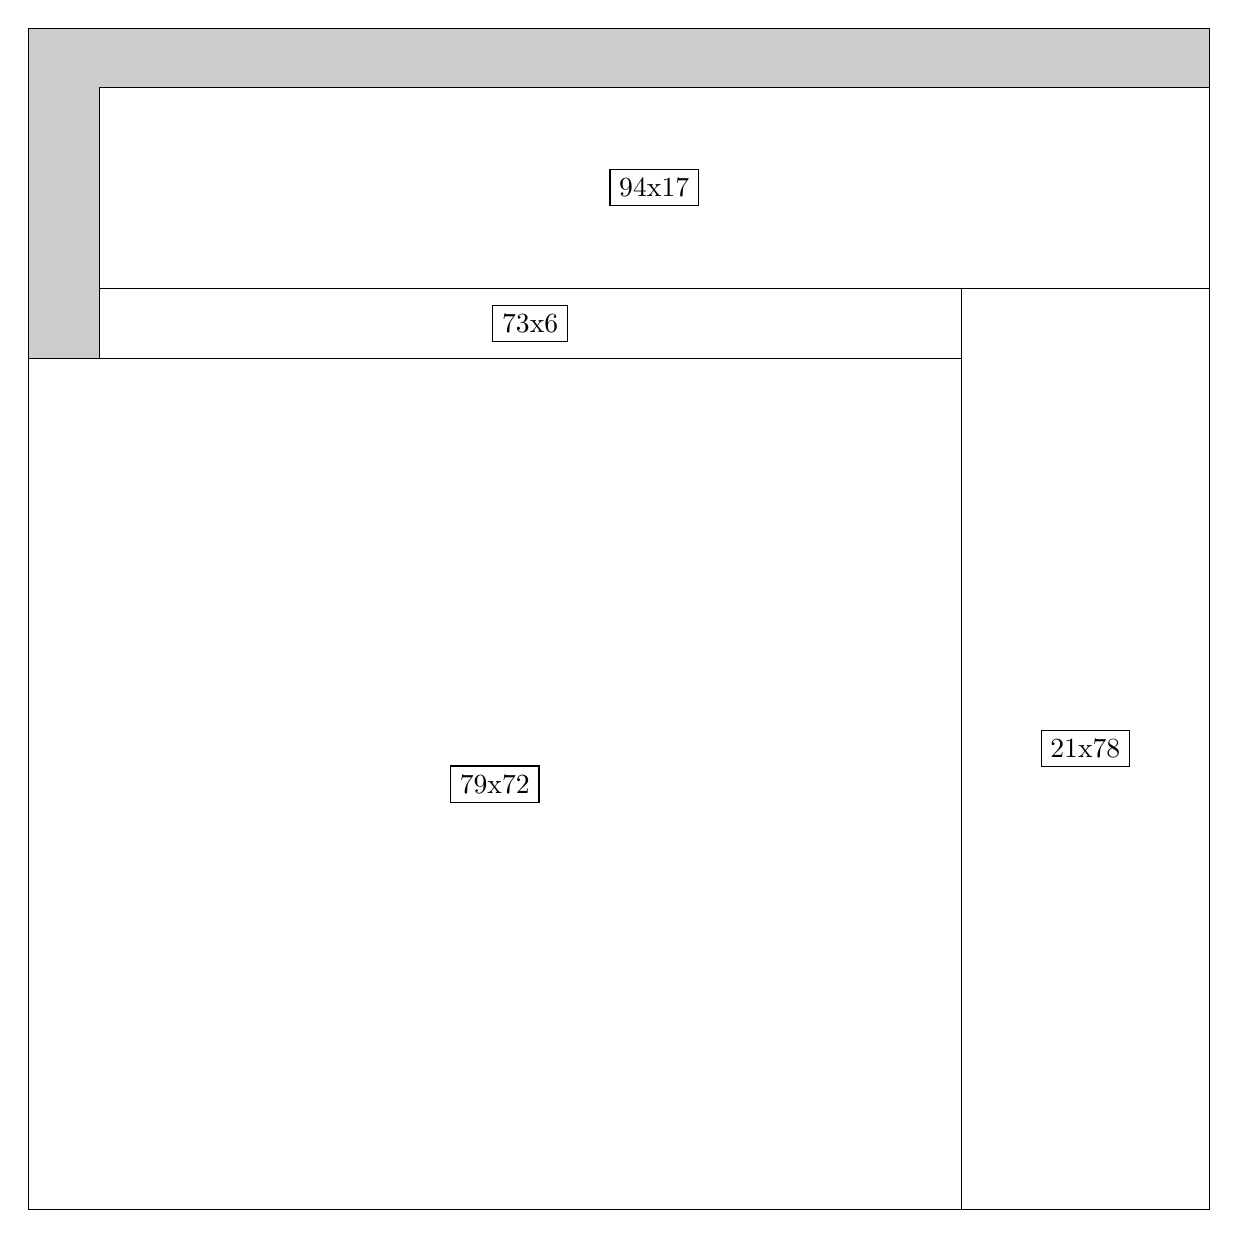
\begin{tikzpicture}[shorten >=1pt,scale=1.0,every node/.style={scale=1.0},->]
\tikzstyle{vertex}=[circle,fill=black!25,minimum size=14pt,inner sep=0pt]
\filldraw[fill=gray!40!white, draw=black] (0,0) rectangle (15.0,15.0);
\foreach \name/\x/\y/\w/\h in {79x72/0.0/0.0/11.85/10.799999999999999,21x78/11.85/0.0/3.15/11.7,94x17/0.8999999999999999/11.7/14.1/2.55,73x6/0.8999999999999999/10.799999999999999/10.95/0.8999999999999999}
\filldraw[fill=white!40!white, draw=black] (\x,\y) rectangle node[draw] (\name) {\name} ++(\w,\h);
\end{tikzpicture}


w =79 , h =72 , x =0 , y =0 , v =5688
\par
w =21 , h =78 , x =79 , y =0 , v =1638
\par
w =94 , h =17 , x =6 , y =78 , v =1598
\par
w =73 , h =6 , x =6 , y =72 , v =438
\par
\newpage


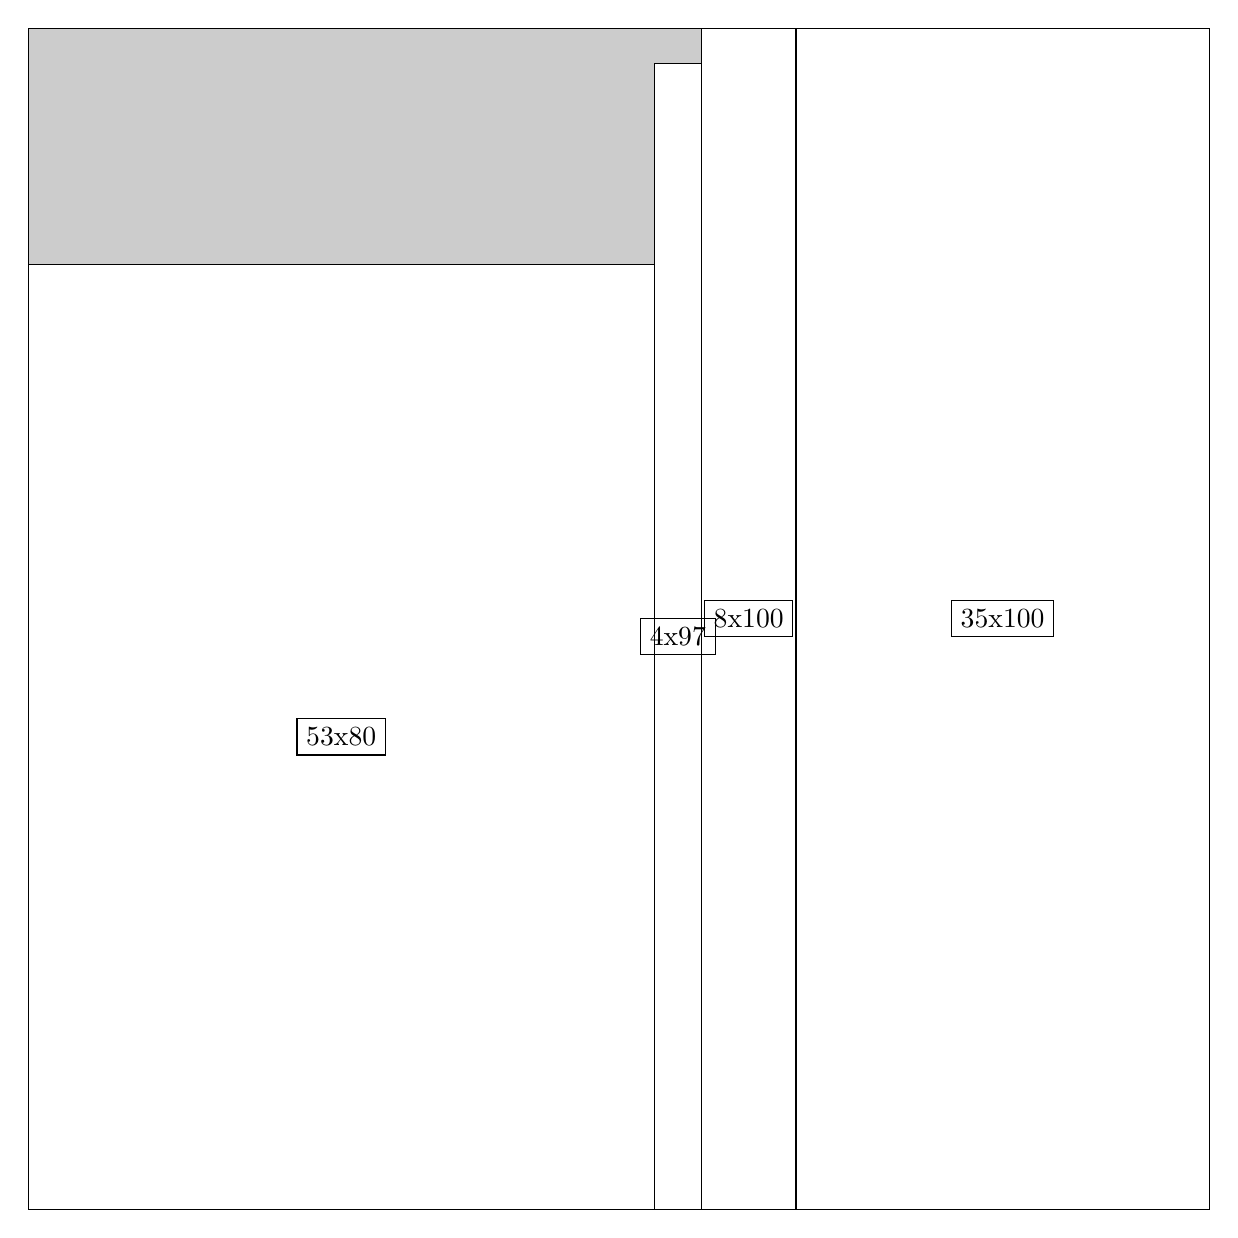
\begin{tikzpicture}[shorten >=1pt,scale=1.0,every node/.style={scale=1.0},->]
\tikzstyle{vertex}=[circle,fill=black!25,minimum size=14pt,inner sep=0pt]
\filldraw[fill=gray!40!white, draw=black] (0,0) rectangle (15.0,15.0);
\foreach \name/\x/\y/\w/\h in {53x80/0.0/0.0/7.949999999999999/12.0,35x100/9.75/0.0/5.25/15.0,8x100/8.549999999999999/0.0/1.2/15.0,4x97/7.949999999999999/0.0/0.6/14.549999999999999}
\filldraw[fill=white!40!white, draw=black] (\x,\y) rectangle node[draw] (\name) {\name} ++(\w,\h);
\end{tikzpicture}


w =53 , h =80 , x =0 , y =0 , v =4240
\par
w =35 , h =100 , x =65 , y =0 , v =3500
\par
w =8 , h =100 , x =57 , y =0 , v =800
\par
w =4 , h =97 , x =53 , y =0 , v =388
\par
\newpage


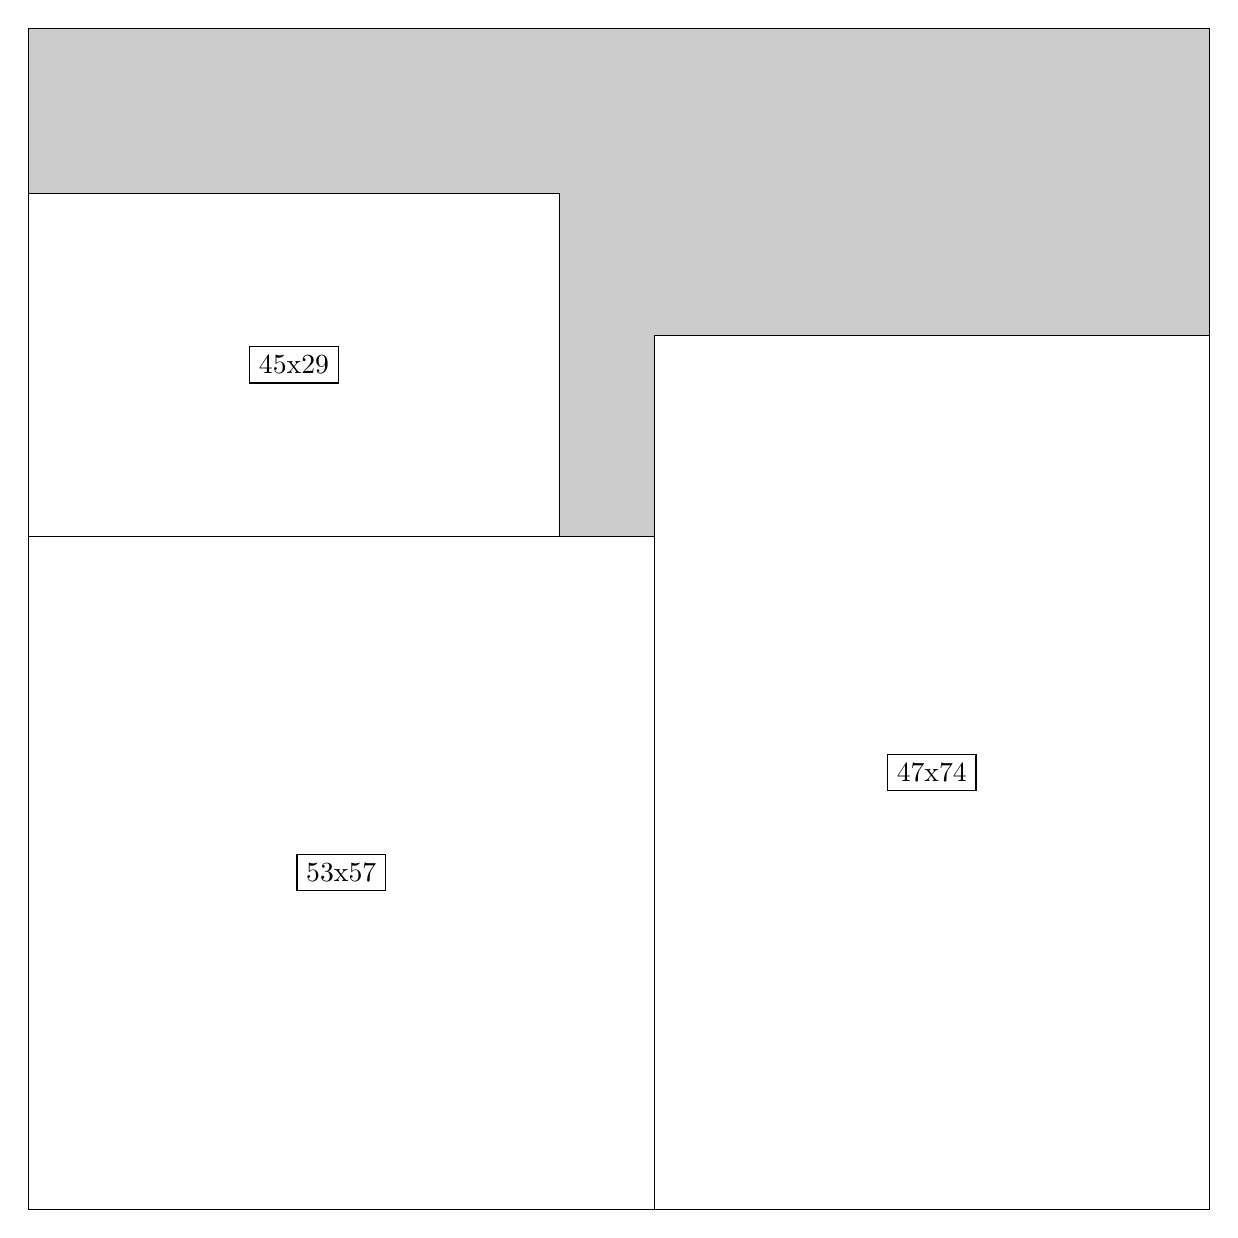
\begin{tikzpicture}[shorten >=1pt,scale=1.0,every node/.style={scale=1.0},->]
\tikzstyle{vertex}=[circle,fill=black!25,minimum size=14pt,inner sep=0pt]
\filldraw[fill=gray!40!white, draw=black] (0,0) rectangle (15.0,15.0);
\foreach \name/\x/\y/\w/\h in {47x74/7.949999999999999/0.0/7.05/11.1,53x57/0.0/0.0/7.949999999999999/8.549999999999999,45x29/0.0/8.549999999999999/6.75/4.35}
\filldraw[fill=white!40!white, draw=black] (\x,\y) rectangle node[draw] (\name) {\name} ++(\w,\h);
\end{tikzpicture}


w =47 , h =74 , x =53 , y =0 , v =3478
\par
w =53 , h =57 , x =0 , y =0 , v =3021
\par
w =45 , h =29 , x =0 , y =57 , v =1305
\par
\newpage


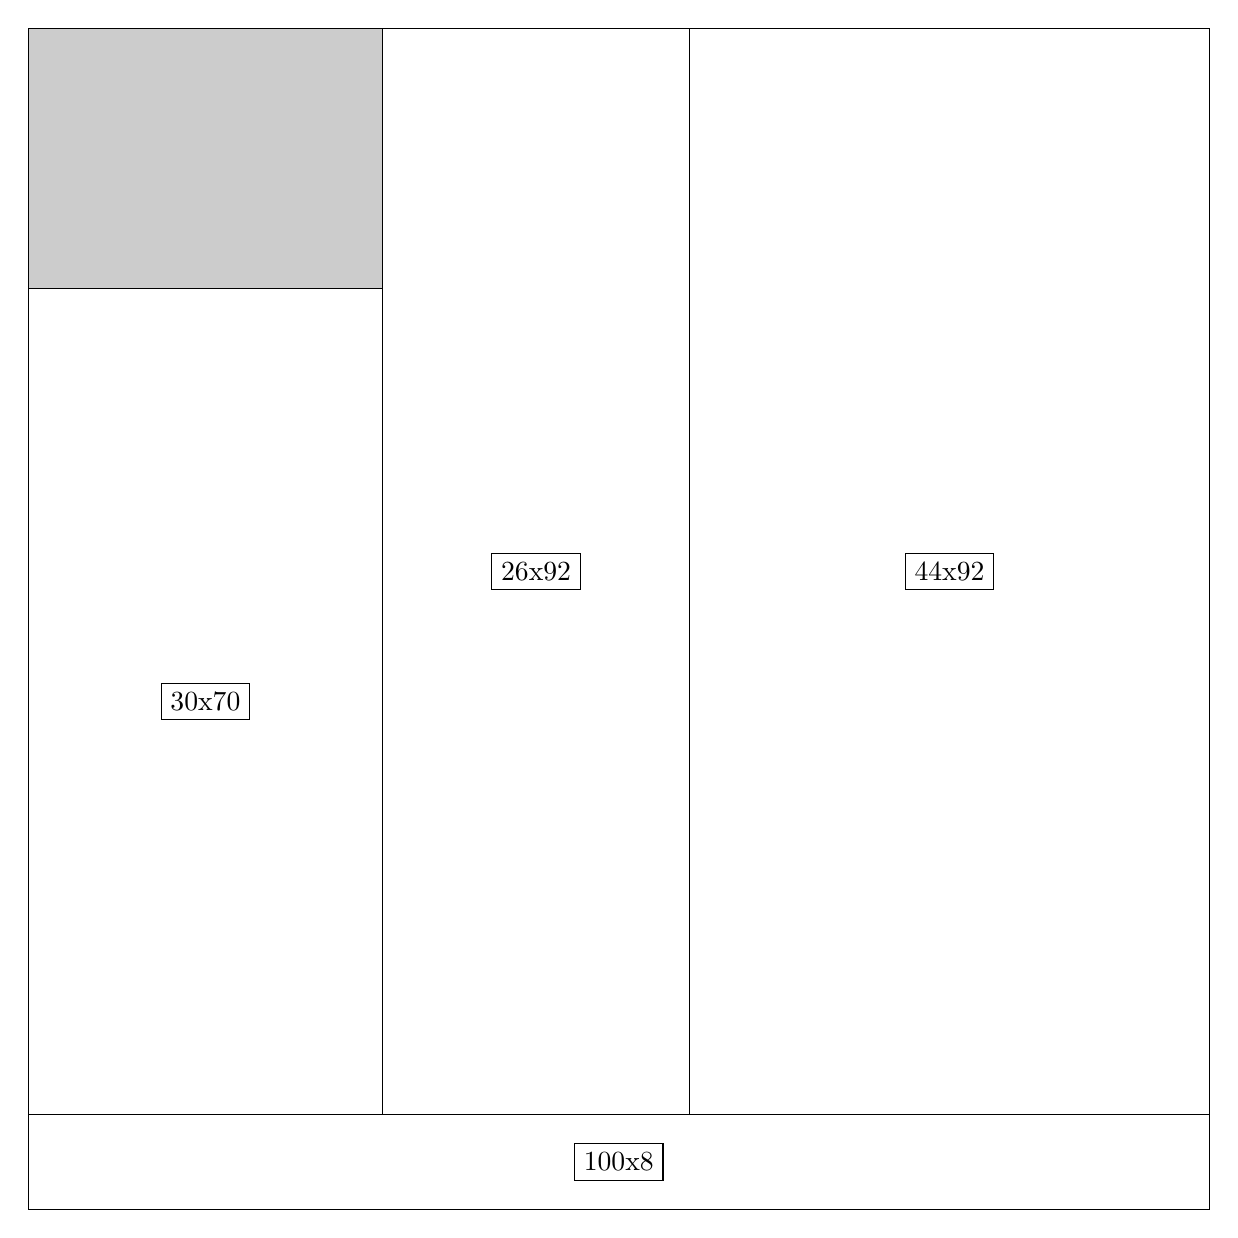
\begin{tikzpicture}[shorten >=1pt,scale=1.0,every node/.style={scale=1.0},->]
\tikzstyle{vertex}=[circle,fill=black!25,minimum size=14pt,inner sep=0pt]
\filldraw[fill=gray!40!white, draw=black] (0,0) rectangle (15.0,15.0);
\foreach \name/\x/\y/\w/\h in {44x92/8.4/1.2/6.6/13.799999999999999,26x92/4.5/1.2/3.9/13.799999999999999,30x70/0.0/1.2/4.5/10.5,100x8/0.0/0.0/15.0/1.2}
\filldraw[fill=white!40!white, draw=black] (\x,\y) rectangle node[draw] (\name) {\name} ++(\w,\h);
\end{tikzpicture}


w =44 , h =92 , x =56 , y =8 , v =4048
\par
w =26 , h =92 , x =30 , y =8 , v =2392
\par
w =30 , h =70 , x =0 , y =8 , v =2100
\par
w =100 , h =8 , x =0 , y =0 , v =800
\par
\newpage


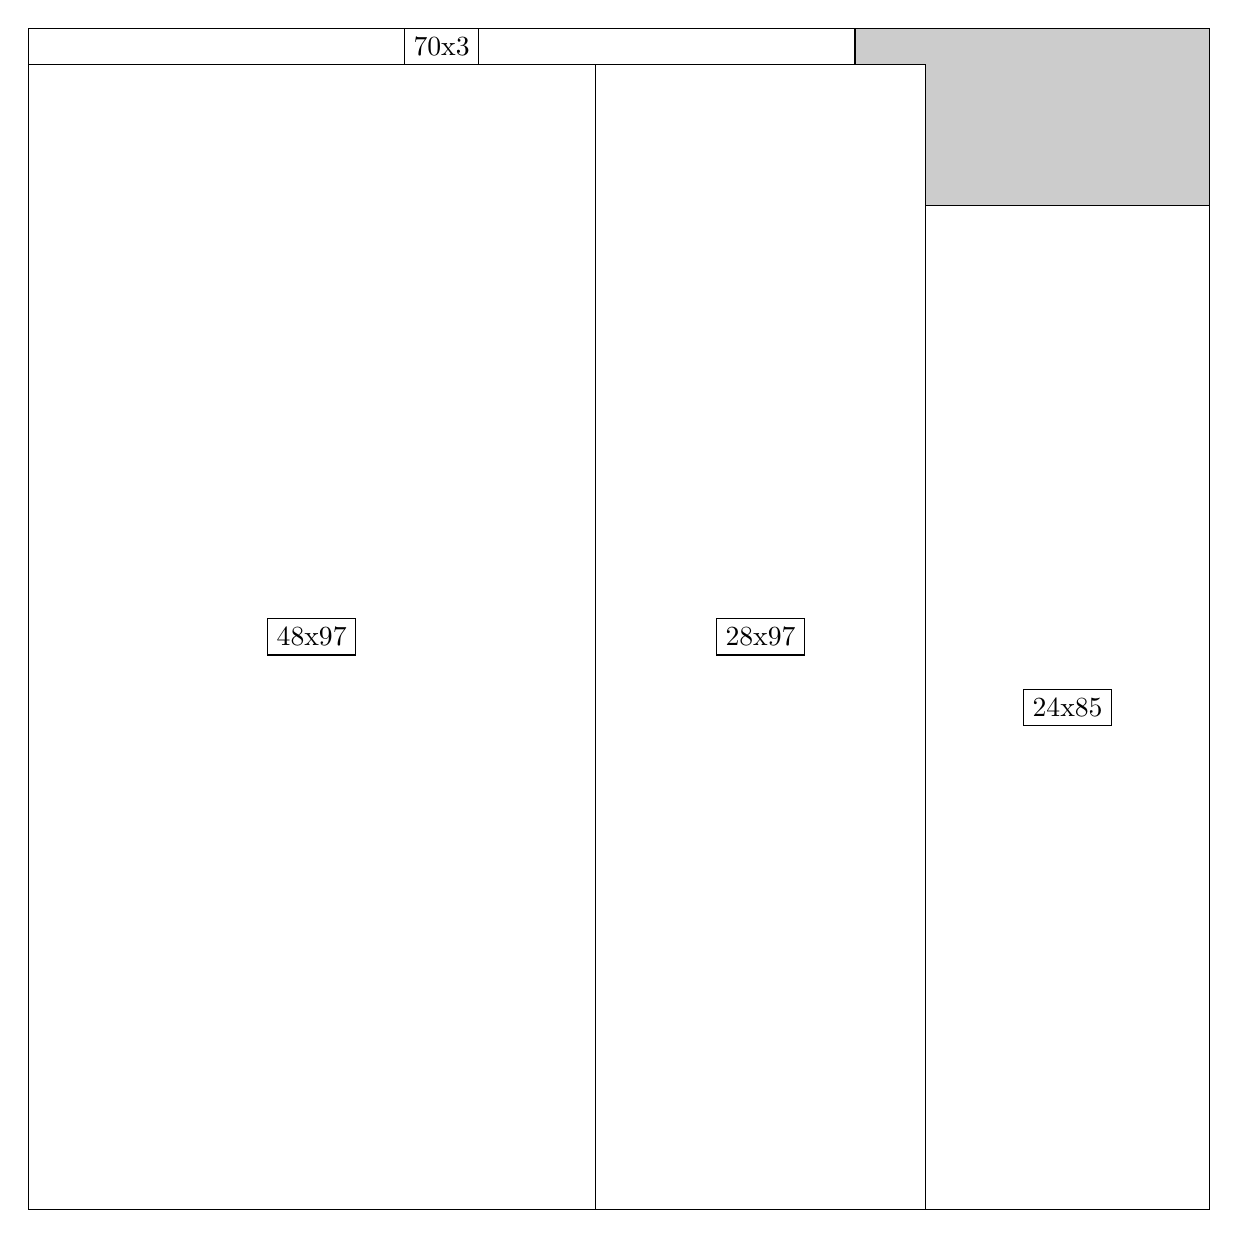
\begin{tikzpicture}[shorten >=1pt,scale=1.0,every node/.style={scale=1.0},->]
\tikzstyle{vertex}=[circle,fill=black!25,minimum size=14pt,inner sep=0pt]
\filldraw[fill=gray!40!white, draw=black] (0,0) rectangle (15.0,15.0);
\foreach \name/\x/\y/\w/\h in {48x97/0.0/0.0/7.199999999999999/14.549999999999999,28x97/7.199999999999999/0.0/4.2/14.549999999999999,24x85/11.4/0.0/3.5999999999999996/12.75,70x3/0.0/14.549999999999999/10.5/0.44999999999999996}
\filldraw[fill=white!40!white, draw=black] (\x,\y) rectangle node[draw] (\name) {\name} ++(\w,\h);
\end{tikzpicture}


w =48 , h =97 , x =0 , y =0 , v =4656
\par
w =28 , h =97 , x =48 , y =0 , v =2716
\par
w =24 , h =85 , x =76 , y =0 , v =2040
\par
w =70 , h =3 , x =0 , y =97 , v =210
\par
\newpage


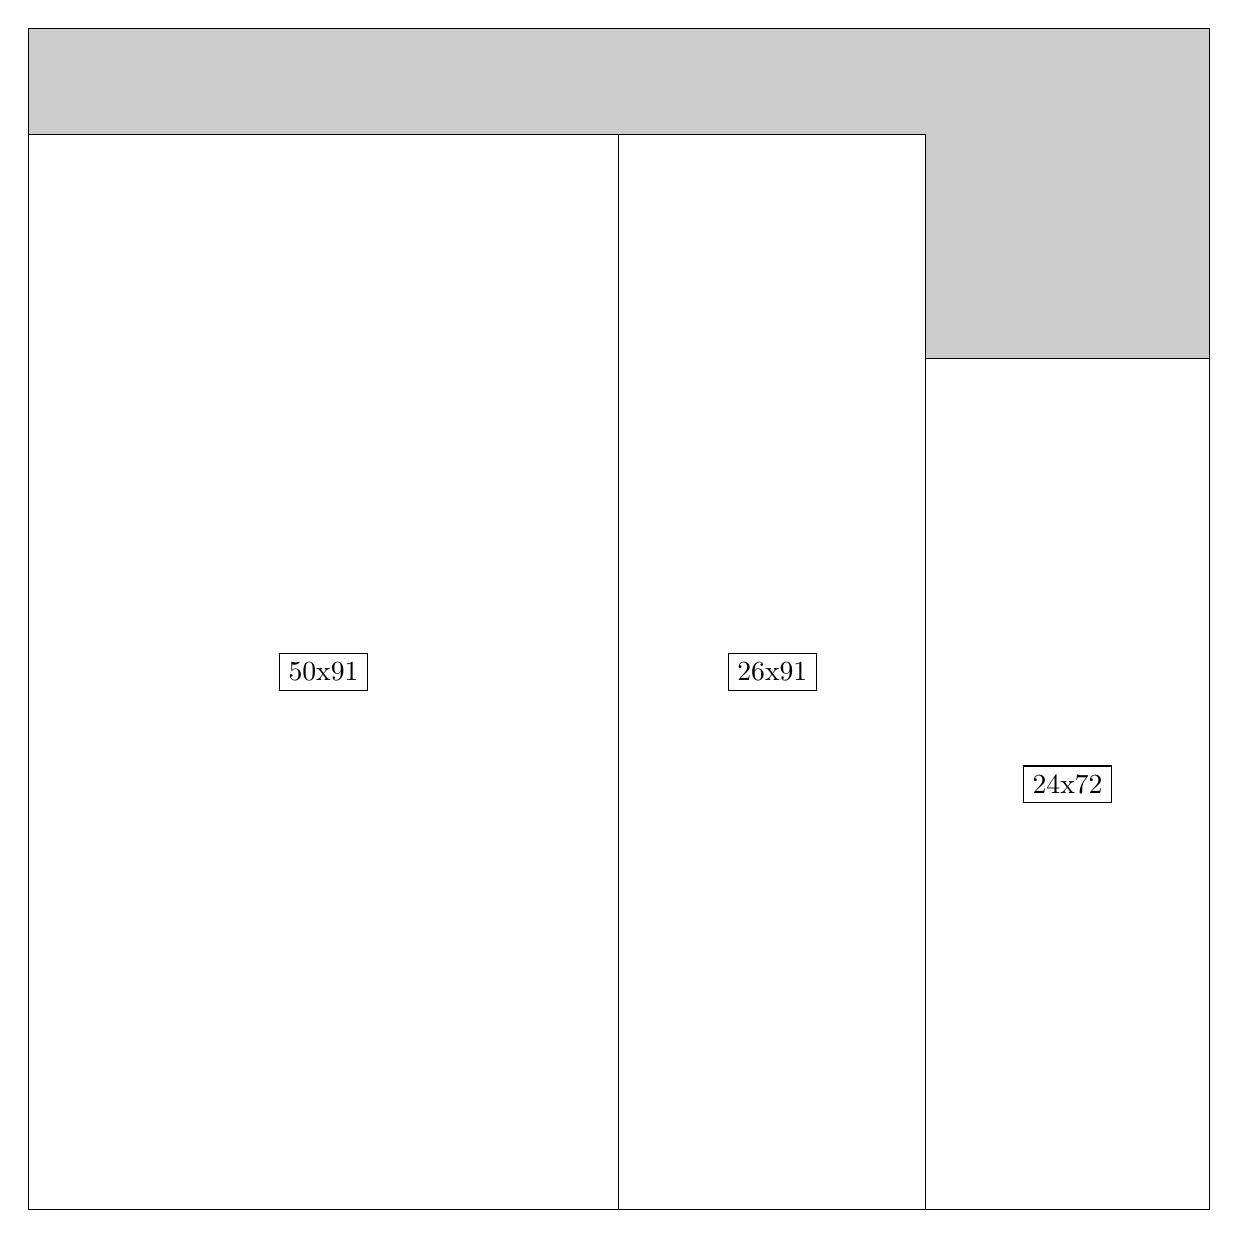
\begin{tikzpicture}[shorten >=1pt,scale=1.0,every node/.style={scale=1.0},->]
\tikzstyle{vertex}=[circle,fill=black!25,minimum size=14pt,inner sep=0pt]
\filldraw[fill=gray!40!white, draw=black] (0,0) rectangle (15.0,15.0);
\foreach \name/\x/\y/\w/\h in {50x91/0.0/0.0/7.5/13.65,26x91/7.5/0.0/3.9/13.65,24x72/11.4/0.0/3.5999999999999996/10.799999999999999}
\filldraw[fill=white!40!white, draw=black] (\x,\y) rectangle node[draw] (\name) {\name} ++(\w,\h);
\end{tikzpicture}


w =50 , h =91 , x =0 , y =0 , v =4550
\par
w =26 , h =91 , x =50 , y =0 , v =2366
\par
w =24 , h =72 , x =76 , y =0 , v =1728
\par
\newpage


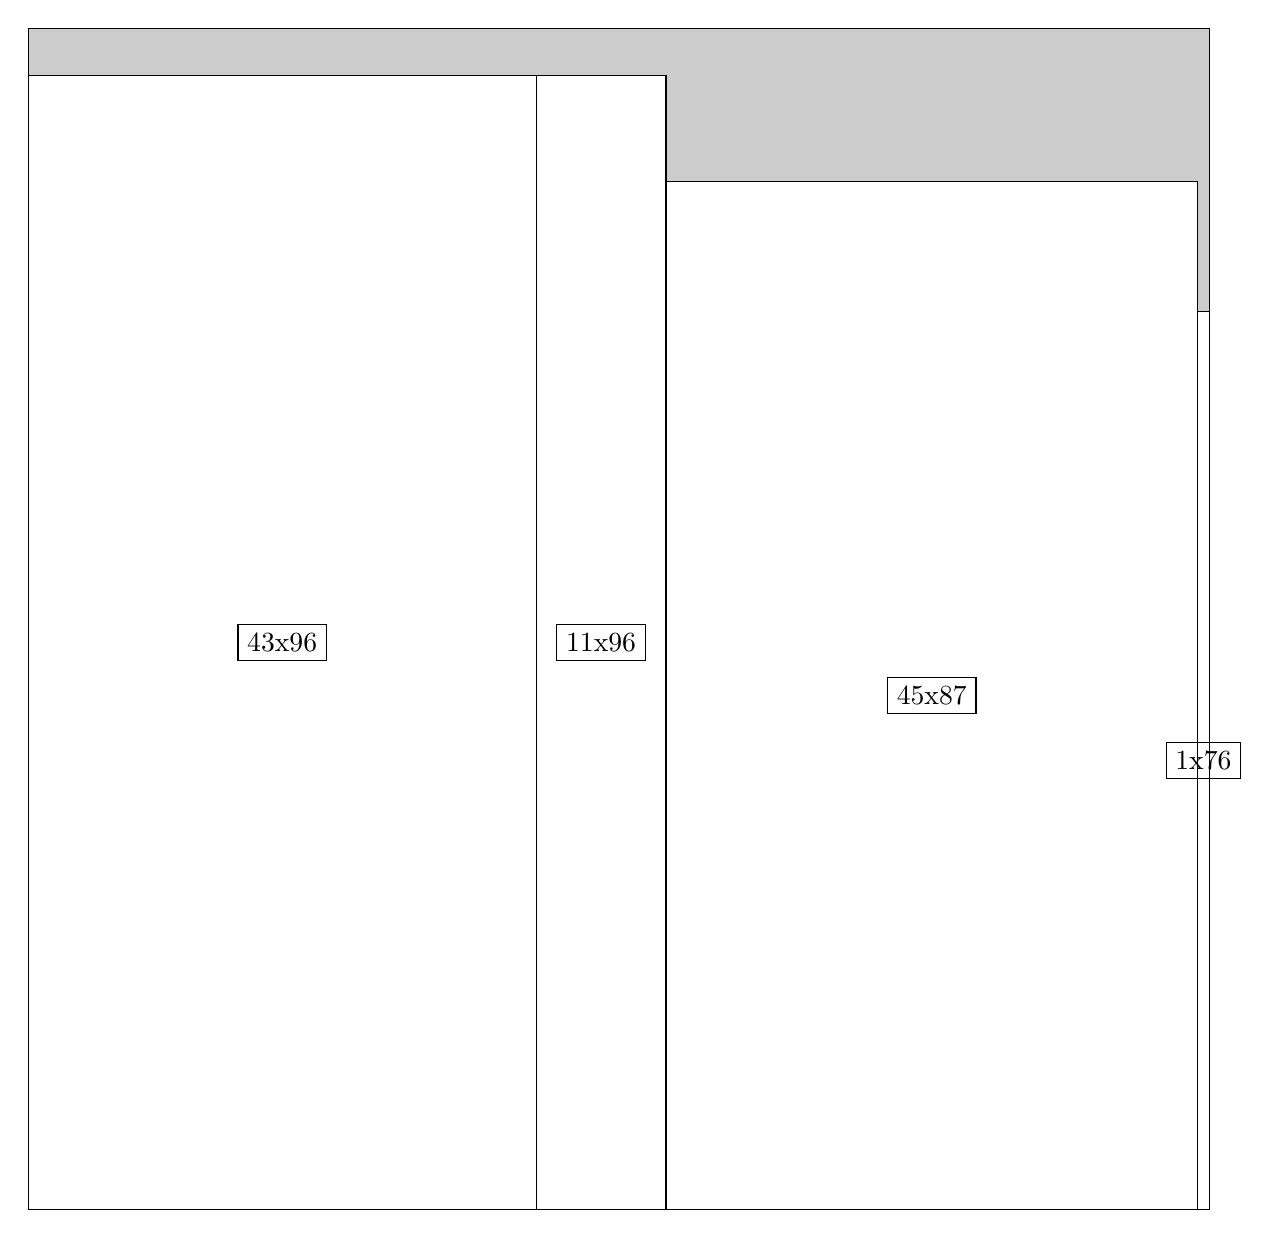
\begin{tikzpicture}[shorten >=1pt,scale=1.0,every node/.style={scale=1.0},->]
\tikzstyle{vertex}=[circle,fill=black!25,minimum size=14pt,inner sep=0pt]
\filldraw[fill=gray!40!white, draw=black] (0,0) rectangle (15.0,15.0);
\foreach \name/\x/\y/\w/\h in {43x96/0.0/0.0/6.45/14.399999999999999,45x87/8.1/0.0/6.75/13.049999999999999,11x96/6.45/0.0/1.65/14.399999999999999,1x76/14.85/0.0/0.15/11.4}
\filldraw[fill=white!40!white, draw=black] (\x,\y) rectangle node[draw] (\name) {\name} ++(\w,\h);
\end{tikzpicture}


w =43 , h =96 , x =0 , y =0 , v =4128
\par
w =45 , h =87 , x =54 , y =0 , v =3915
\par
w =11 , h =96 , x =43 , y =0 , v =1056
\par
w =1 , h =76 , x =99 , y =0 , v =76
\par
\newpage


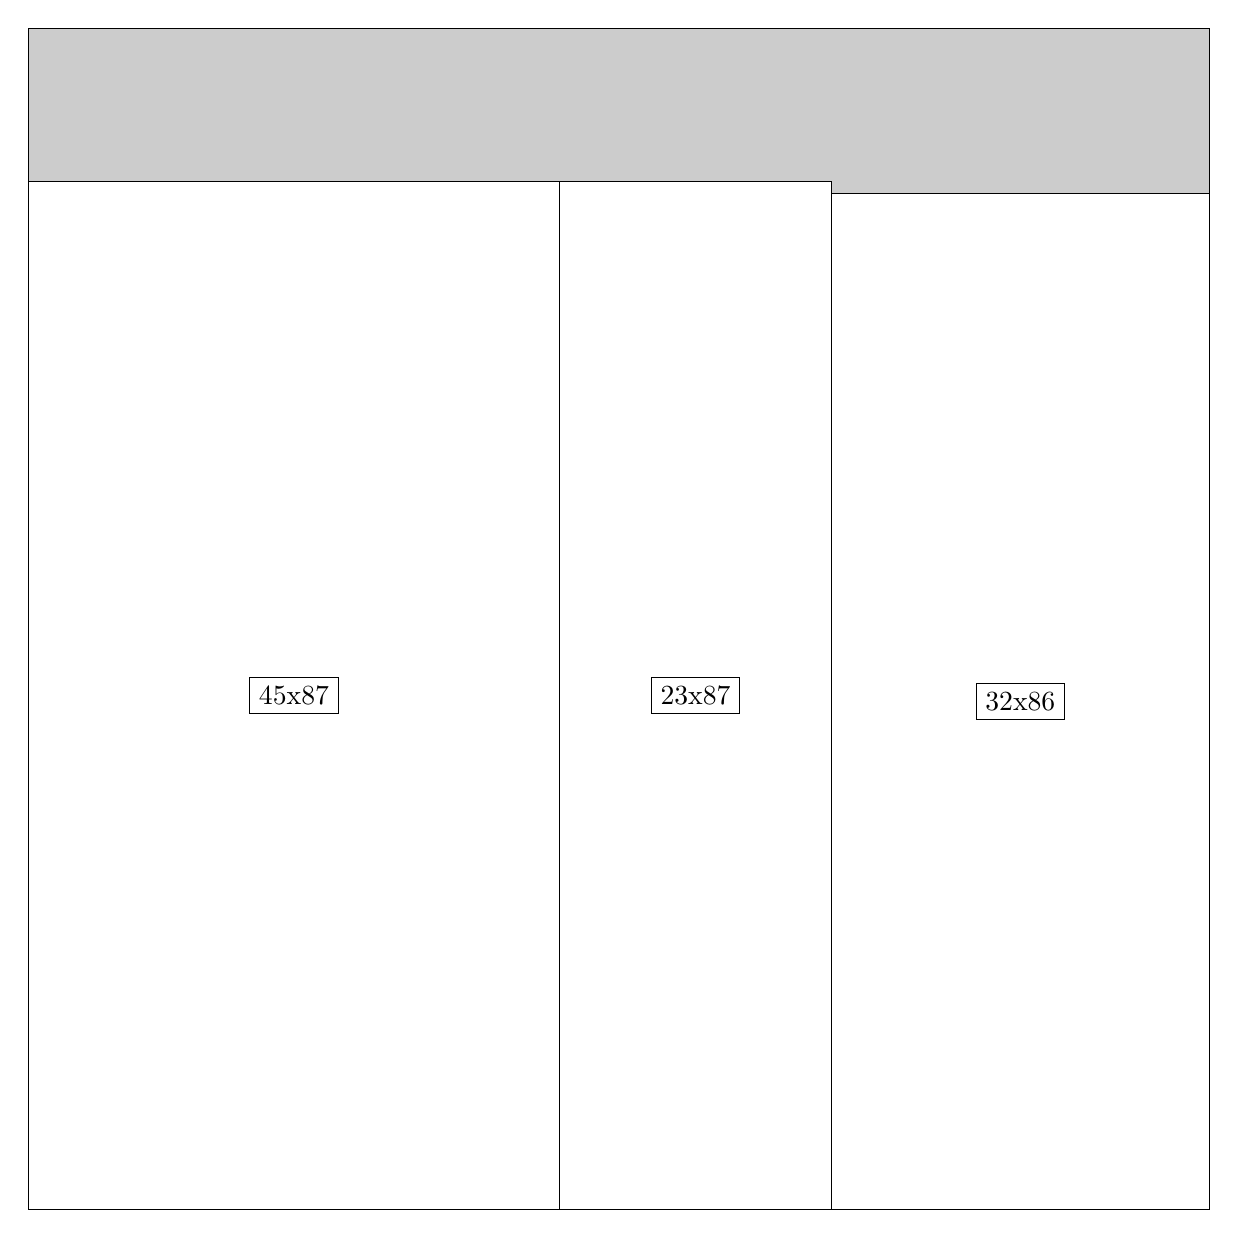
\begin{tikzpicture}[shorten >=1pt,scale=1.0,every node/.style={scale=1.0},->]
\tikzstyle{vertex}=[circle,fill=black!25,minimum size=14pt,inner sep=0pt]
\filldraw[fill=gray!40!white, draw=black] (0,0) rectangle (15.0,15.0);
\foreach \name/\x/\y/\w/\h in {45x87/0.0/0.0/6.75/13.049999999999999,32x86/10.2/0.0/4.8/12.9,23x87/6.75/0.0/3.4499999999999997/13.049999999999999}
\filldraw[fill=white!40!white, draw=black] (\x,\y) rectangle node[draw] (\name) {\name} ++(\w,\h);
\end{tikzpicture}


w =45 , h =87 , x =0 , y =0 , v =3915
\par
w =32 , h =86 , x =68 , y =0 , v =2752
\par
w =23 , h =87 , x =45 , y =0 , v =2001
\par
\newpage


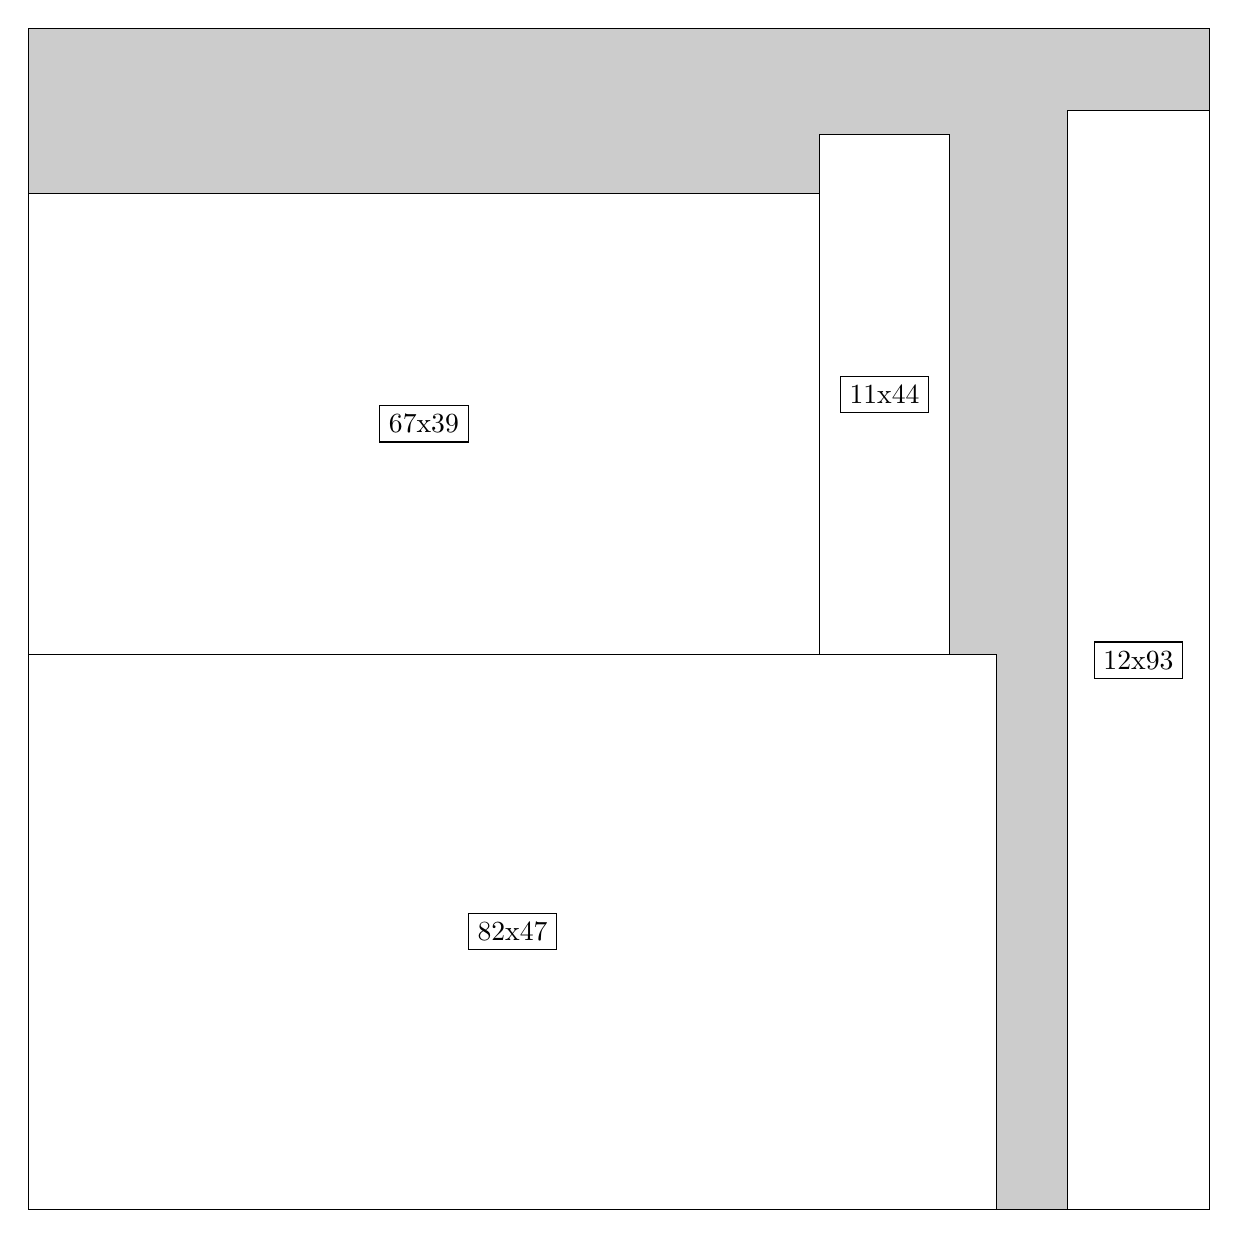
\begin{tikzpicture}[shorten >=1pt,scale=1.0,every node/.style={scale=1.0},->]
\tikzstyle{vertex}=[circle,fill=black!25,minimum size=14pt,inner sep=0pt]
\filldraw[fill=gray!40!white, draw=black] (0,0) rectangle (15.0,15.0);
\foreach \name/\x/\y/\w/\h in {82x47/0.0/0.0/12.299999999999999/7.05,67x39/0.0/7.05/10.049999999999999/5.85,12x93/13.2/0.0/1.7999999999999998/13.95,11x44/10.049999999999999/7.05/1.65/6.6}
\filldraw[fill=white!40!white, draw=black] (\x,\y) rectangle node[draw] (\name) {\name} ++(\w,\h);
\end{tikzpicture}


w =82 , h =47 , x =0 , y =0 , v =3854
\par
w =67 , h =39 , x =0 , y =47 , v =2613
\par
w =12 , h =93 , x =88 , y =0 , v =1116
\par
w =11 , h =44 , x =67 , y =47 , v =484
\par
\newpage


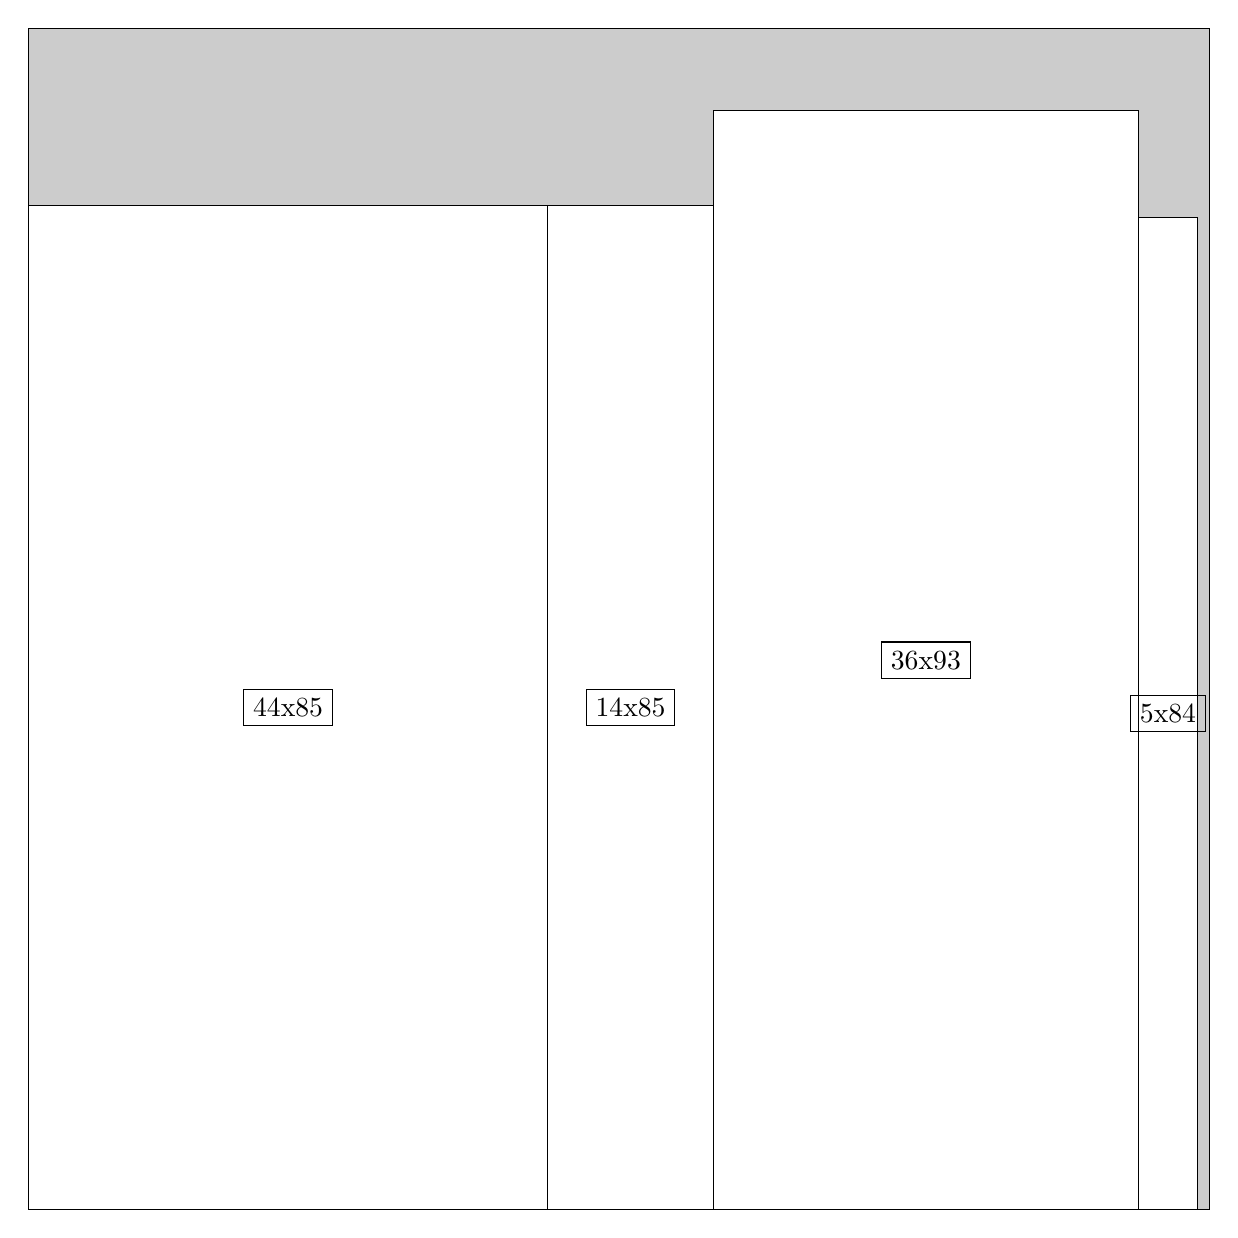
\begin{tikzpicture}[shorten >=1pt,scale=1.0,every node/.style={scale=1.0},->]
\tikzstyle{vertex}=[circle,fill=black!25,minimum size=14pt,inner sep=0pt]
\filldraw[fill=gray!40!white, draw=black] (0,0) rectangle (15.0,15.0);
\foreach \name/\x/\y/\w/\h in {44x85/0.0/0.0/6.6/12.75,36x93/8.7/0.0/5.3999999999999995/13.95,14x85/6.6/0.0/2.1/12.75,5x84/14.1/0.0/0.75/12.6}
\filldraw[fill=white!40!white, draw=black] (\x,\y) rectangle node[draw] (\name) {\name} ++(\w,\h);
\end{tikzpicture}


w =44 , h =85 , x =0 , y =0 , v =3740
\par
w =36 , h =93 , x =58 , y =0 , v =3348
\par
w =14 , h =85 , x =44 , y =0 , v =1190
\par
w =5 , h =84 , x =94 , y =0 , v =420
\par
\newpage


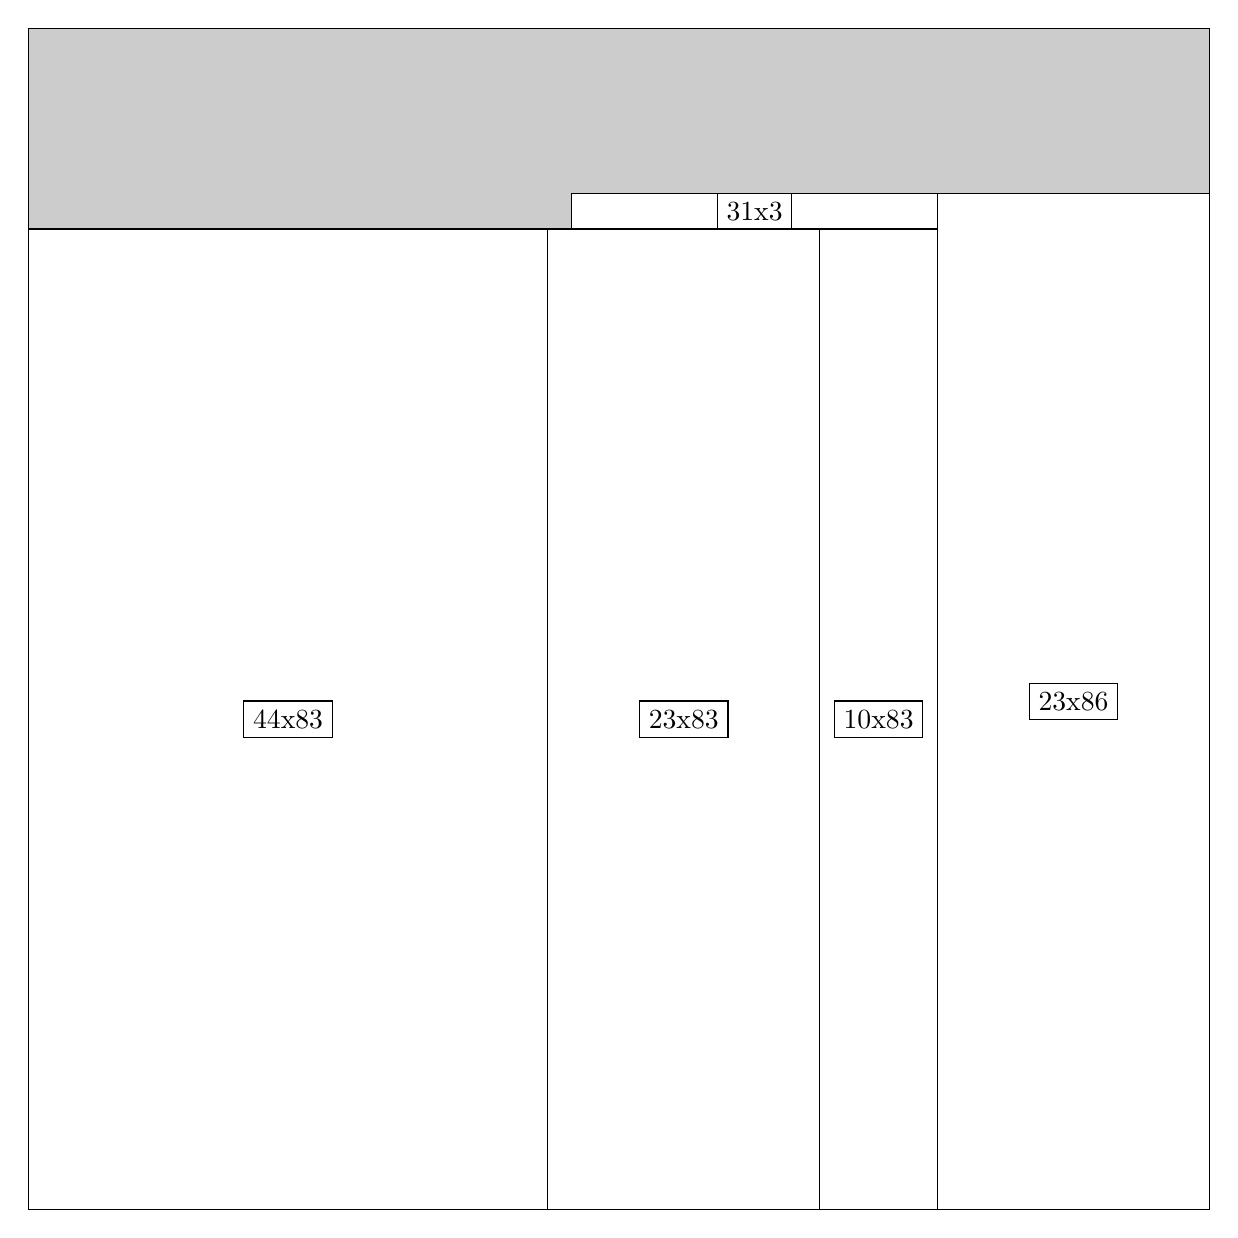
\begin{tikzpicture}[shorten >=1pt,scale=1.0,every node/.style={scale=1.0},->]
\tikzstyle{vertex}=[circle,fill=black!25,minimum size=14pt,inner sep=0pt]
\filldraw[fill=gray!40!white, draw=black] (0,0) rectangle (15.0,15.0);
\foreach \name/\x/\y/\w/\h in {44x83/0.0/0.0/6.6/12.45,23x86/11.549999999999999/0.0/3.4499999999999997/12.9,23x83/6.6/0.0/3.4499999999999997/12.45,10x83/10.049999999999999/0.0/1.5/12.45,31x3/6.8999999999999995/12.45/4.6499999999999995/0.44999999999999996}
\filldraw[fill=white!40!white, draw=black] (\x,\y) rectangle node[draw] (\name) {\name} ++(\w,\h);
\end{tikzpicture}


w =44 , h =83 , x =0 , y =0 , v =3652
\par
w =23 , h =86 , x =77 , y =0 , v =1978
\par
w =23 , h =83 , x =44 , y =0 , v =1909
\par
w =10 , h =83 , x =67 , y =0 , v =830
\par
w =31 , h =3 , x =46 , y =83 , v =93
\par
\newpage


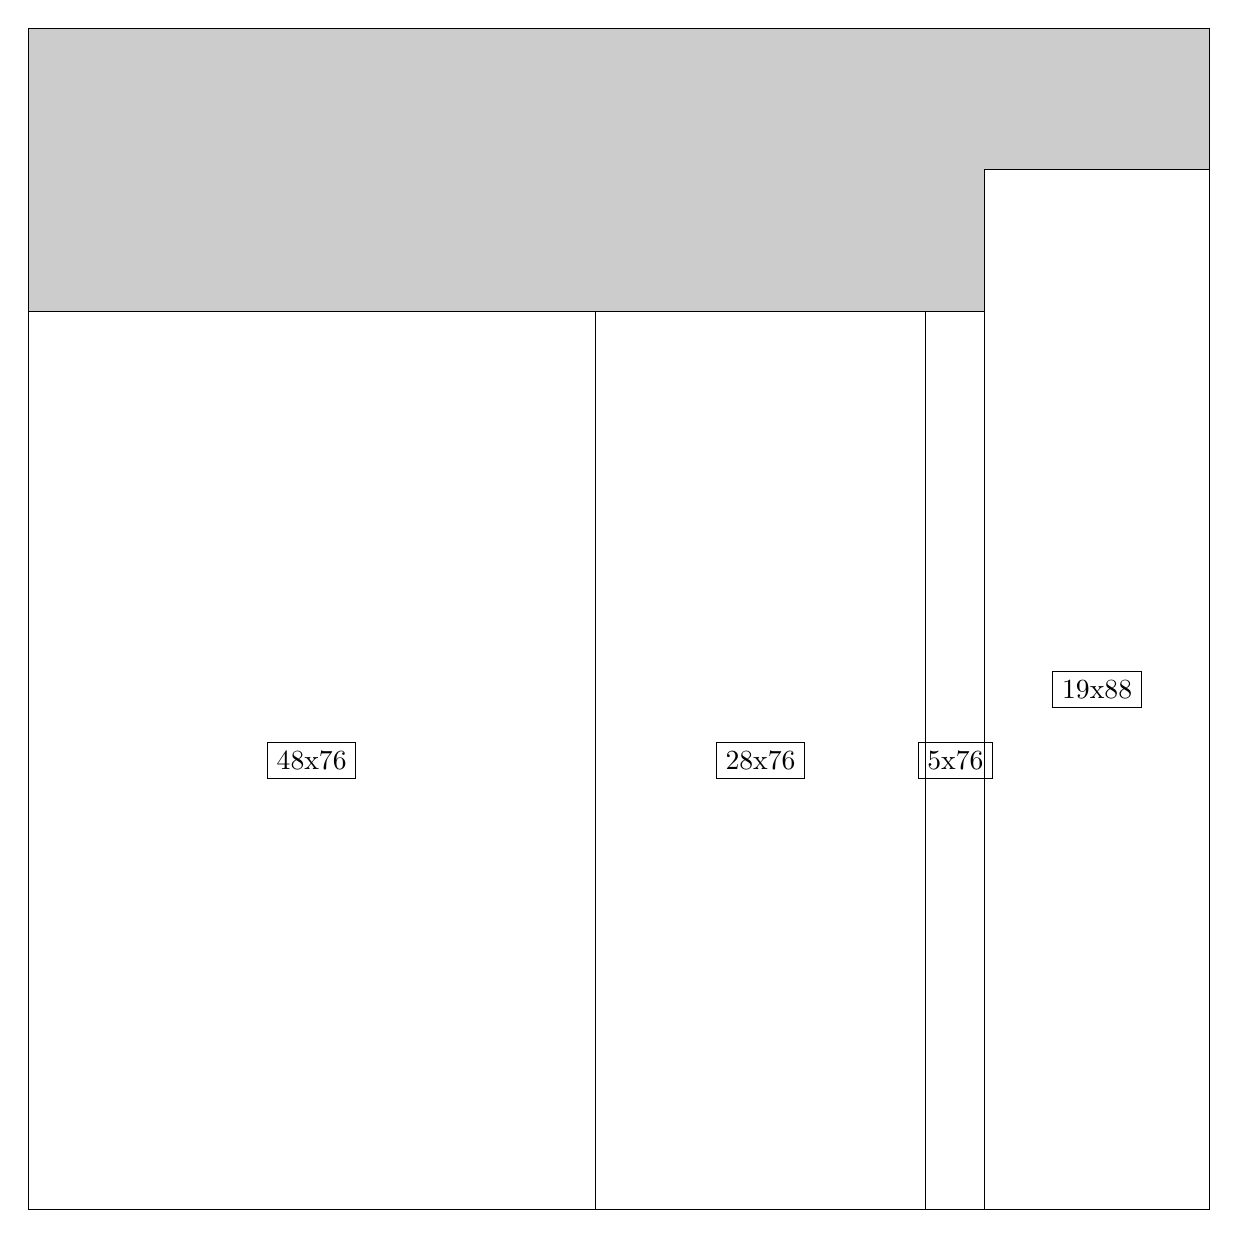
\begin{tikzpicture}[shorten >=1pt,scale=1.0,every node/.style={scale=1.0},->]
\tikzstyle{vertex}=[circle,fill=black!25,minimum size=14pt,inner sep=0pt]
\filldraw[fill=gray!40!white, draw=black] (0,0) rectangle (15.0,15.0);
\foreach \name/\x/\y/\w/\h in {48x76/0.0/0.0/7.199999999999999/11.4,28x76/7.199999999999999/0.0/4.2/11.4,19x88/12.15/0.0/2.85/13.2,5x76/11.4/0.0/0.75/11.4}
\filldraw[fill=white!40!white, draw=black] (\x,\y) rectangle node[draw] (\name) {\name} ++(\w,\h);
\end{tikzpicture}


w =48 , h =76 , x =0 , y =0 , v =3648
\par
w =28 , h =76 , x =48 , y =0 , v =2128
\par
w =19 , h =88 , x =81 , y =0 , v =1672
\par
w =5 , h =76 , x =76 , y =0 , v =380
\par
\newpage


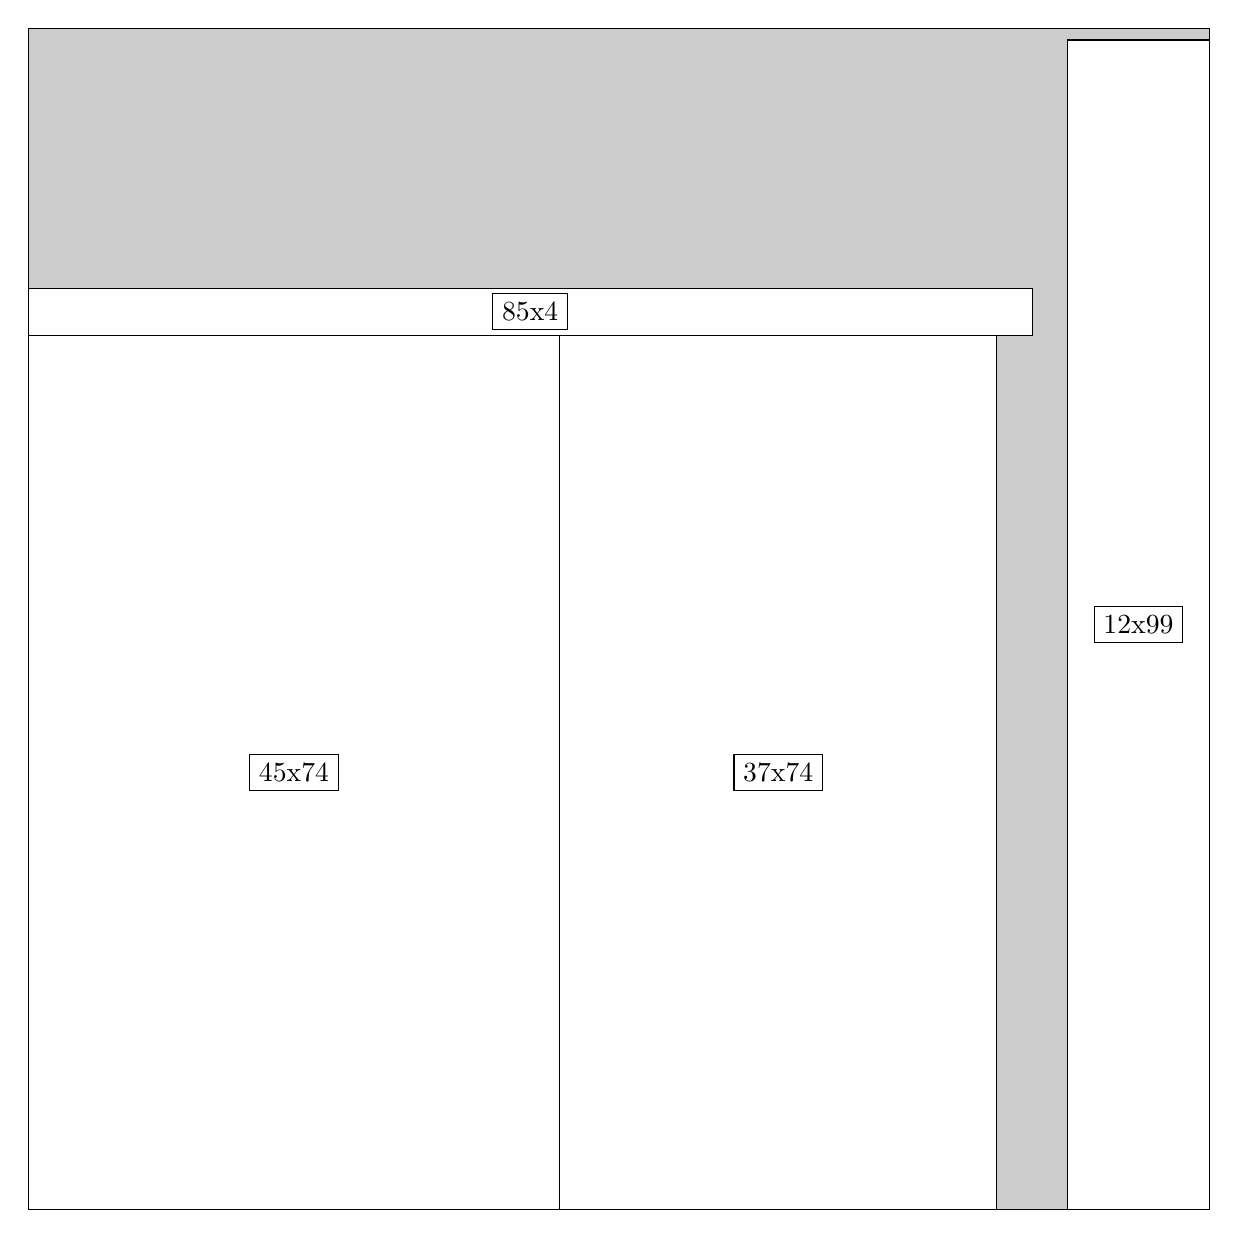
\begin{tikzpicture}[shorten >=1pt,scale=1.0,every node/.style={scale=1.0},->]
\tikzstyle{vertex}=[circle,fill=black!25,minimum size=14pt,inner sep=0pt]
\filldraw[fill=gray!40!white, draw=black] (0,0) rectangle (15.0,15.0);
\foreach \name/\x/\y/\w/\h in {45x74/0.0/0.0/6.75/11.1,37x74/6.75/0.0/5.55/11.1,12x99/13.2/0.0/1.7999999999999998/14.85,85x4/0.0/11.1/12.75/0.6}
\filldraw[fill=white!40!white, draw=black] (\x,\y) rectangle node[draw] (\name) {\name} ++(\w,\h);
\end{tikzpicture}


w =45 , h =74 , x =0 , y =0 , v =3330
\par
w =37 , h =74 , x =45 , y =0 , v =2738
\par
w =12 , h =99 , x =88 , y =0 , v =1188
\par
w =85 , h =4 , x =0 , y =74 , v =340
\par
\newpage


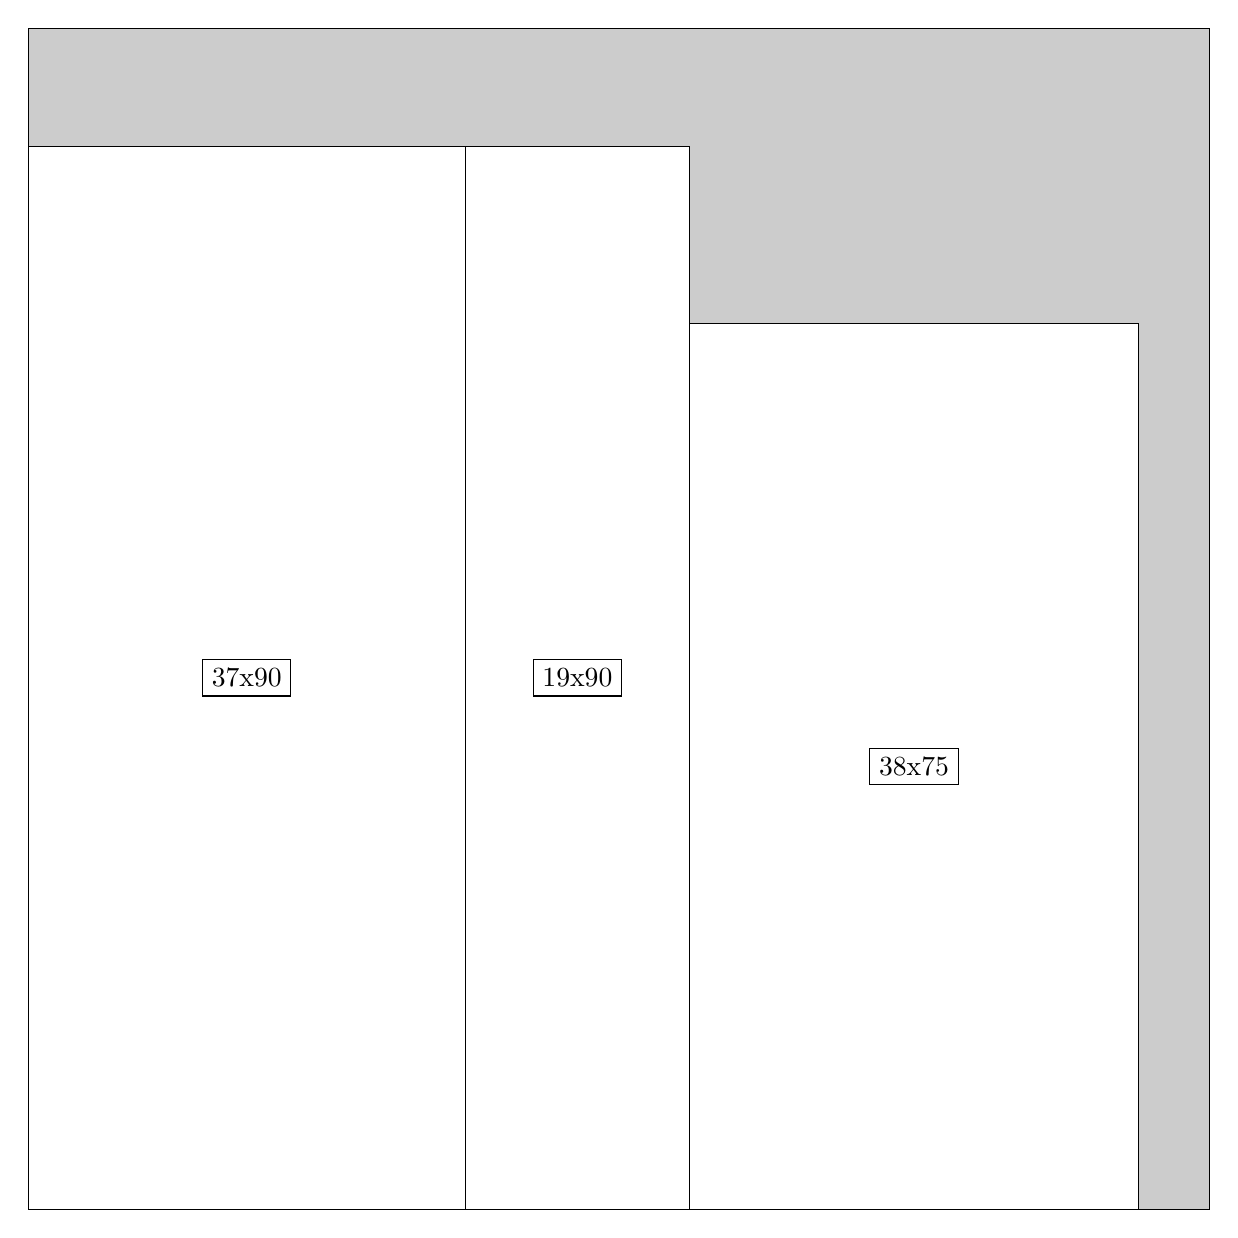
\begin{tikzpicture}[shorten >=1pt,scale=1.0,every node/.style={scale=1.0},->]
\tikzstyle{vertex}=[circle,fill=black!25,minimum size=14pt,inner sep=0pt]
\filldraw[fill=gray!40!white, draw=black] (0,0) rectangle (15.0,15.0);
\foreach \name/\x/\y/\w/\h in {37x90/0.0/0.0/5.55/13.5,38x75/8.4/0.0/5.7/11.25,19x90/5.55/0.0/2.85/13.5}
\filldraw[fill=white!40!white, draw=black] (\x,\y) rectangle node[draw] (\name) {\name} ++(\w,\h);
\end{tikzpicture}


w =37 , h =90 , x =0 , y =0 , v =3330
\par
w =38 , h =75 , x =56 , y =0 , v =2850
\par
w =19 , h =90 , x =37 , y =0 , v =1710
\par
\newpage


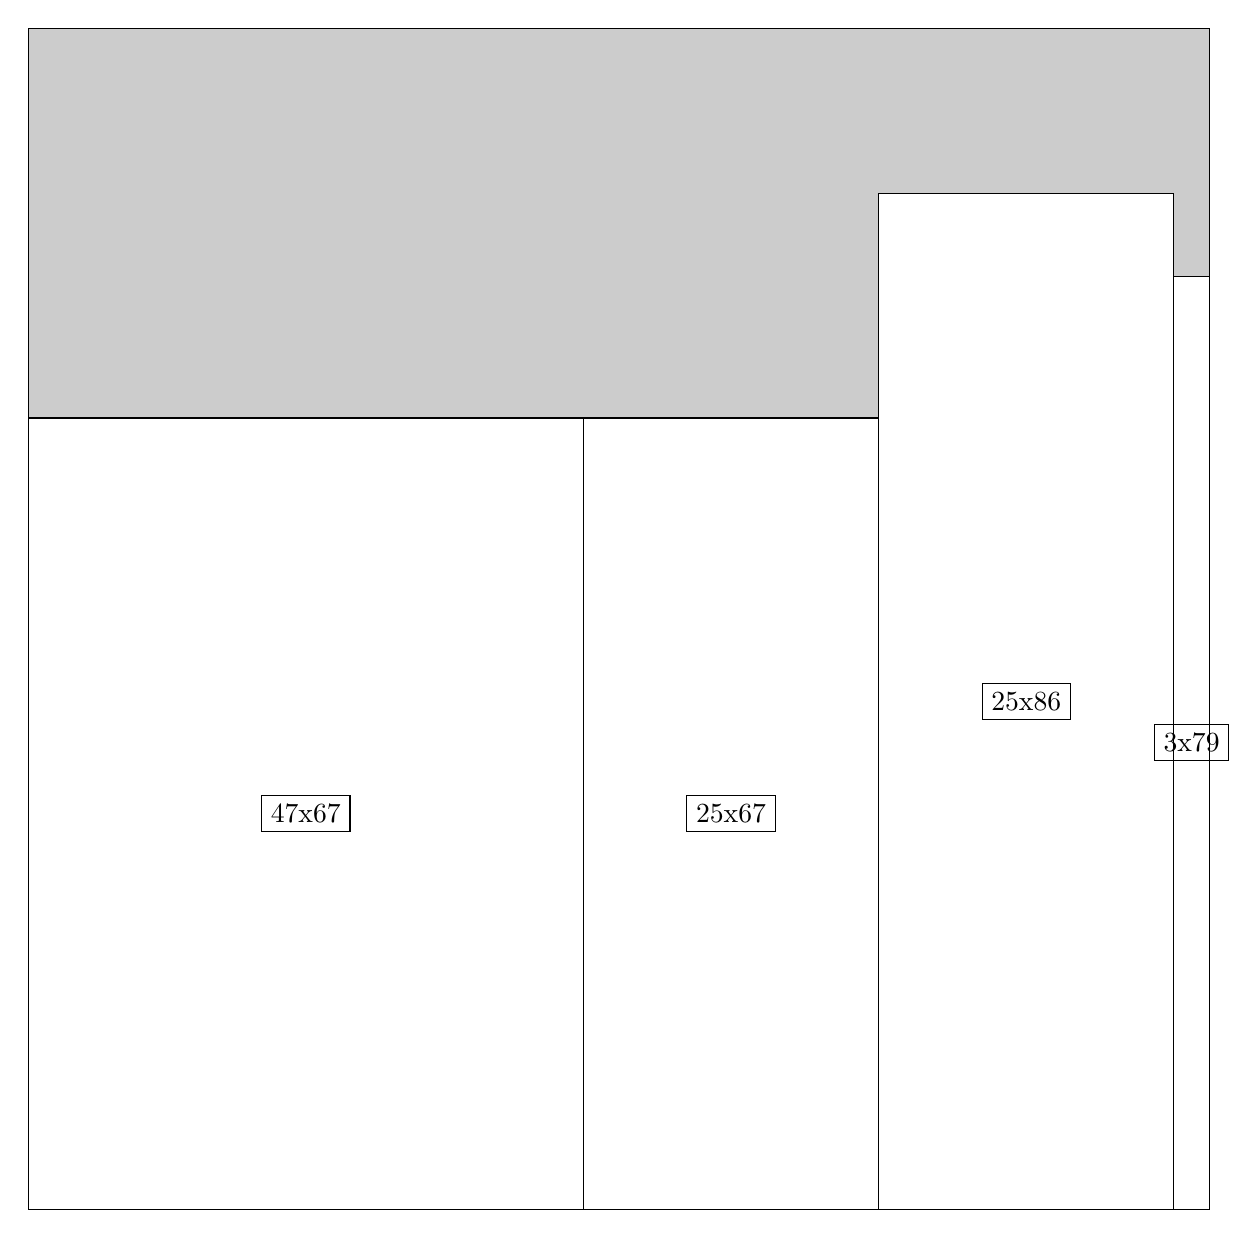
\begin{tikzpicture}[shorten >=1pt,scale=1.0,every node/.style={scale=1.0},->]
\tikzstyle{vertex}=[circle,fill=black!25,minimum size=14pt,inner sep=0pt]
\filldraw[fill=gray!40!white, draw=black] (0,0) rectangle (15.0,15.0);
\foreach \name/\x/\y/\w/\h in {47x67/0.0/0.0/7.05/10.049999999999999,25x86/10.799999999999999/0.0/3.75/12.9,25x67/7.05/0.0/3.75/10.049999999999999,3x79/14.549999999999999/0.0/0.44999999999999996/11.85}
\filldraw[fill=white!40!white, draw=black] (\x,\y) rectangle node[draw] (\name) {\name} ++(\w,\h);
\end{tikzpicture}


w =47 , h =67 , x =0 , y =0 , v =3149
\par
w =25 , h =86 , x =72 , y =0 , v =2150
\par
w =25 , h =67 , x =47 , y =0 , v =1675
\par
w =3 , h =79 , x =97 , y =0 , v =237
\par
\newpage


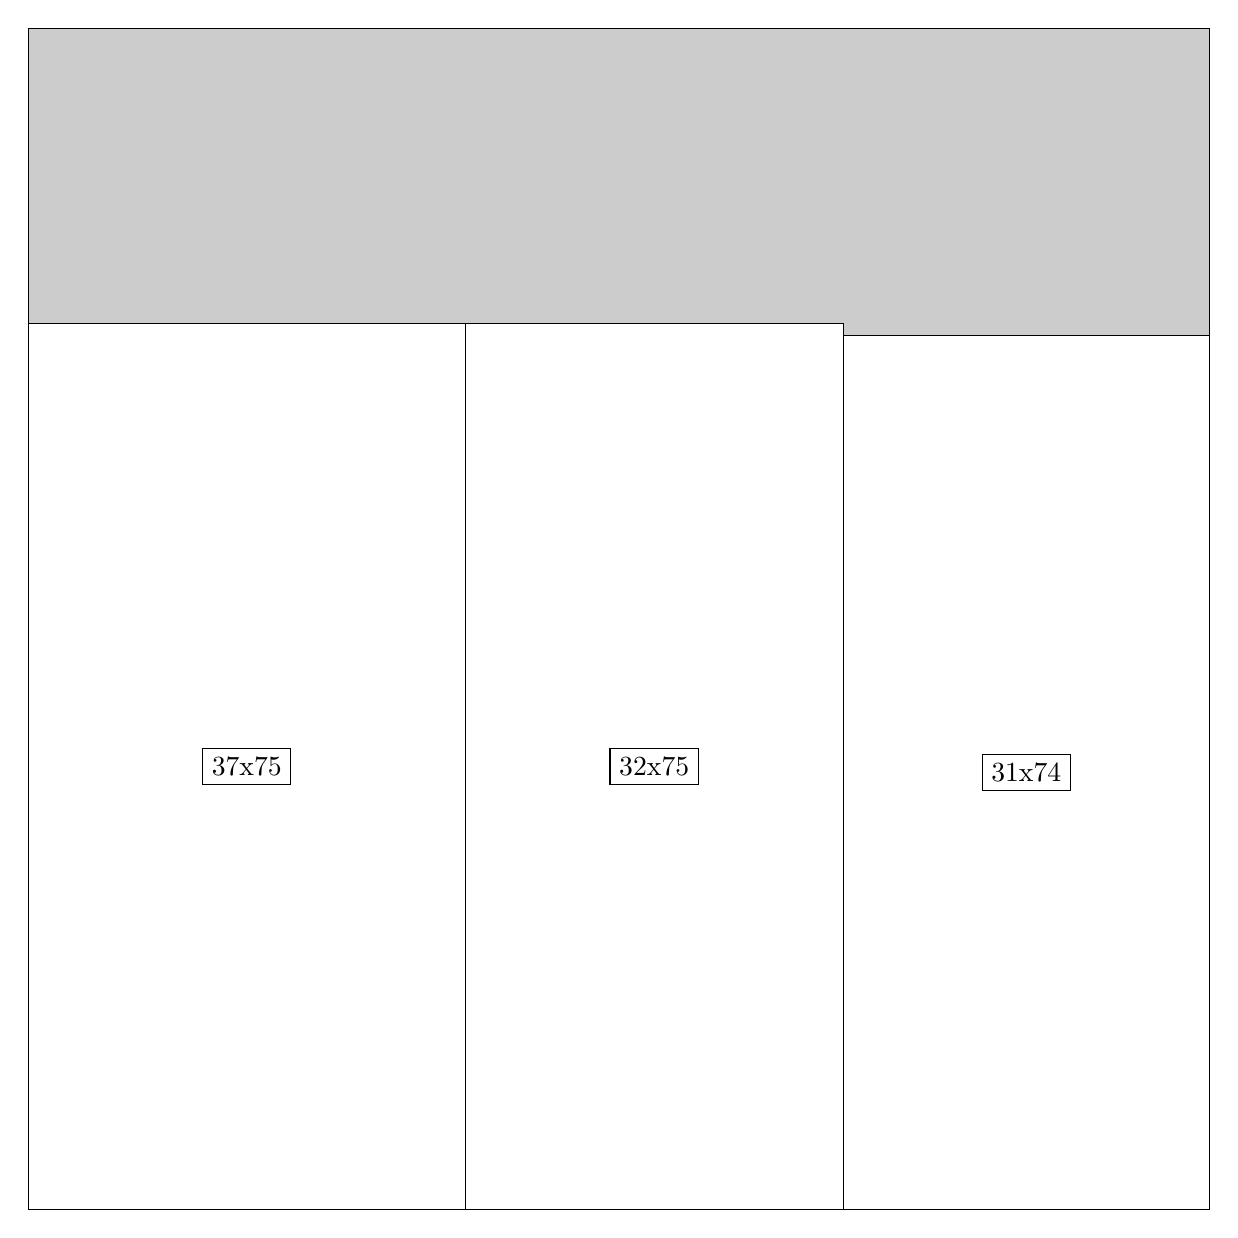
\begin{tikzpicture}[shorten >=1pt,scale=1.0,every node/.style={scale=1.0},->]
\tikzstyle{vertex}=[circle,fill=black!25,minimum size=14pt,inner sep=0pt]
\filldraw[fill=gray!40!white, draw=black] (0,0) rectangle (15.0,15.0);
\foreach \name/\x/\y/\w/\h in {37x75/0.0/0.0/5.55/11.25,32x75/5.55/0.0/4.8/11.25,31x74/10.35/0.0/4.6499999999999995/11.1}
\filldraw[fill=white!40!white, draw=black] (\x,\y) rectangle node[draw] (\name) {\name} ++(\w,\h);
\end{tikzpicture}


w =37 , h =75 , x =0 , y =0 , v =2775
\par
w =32 , h =75 , x =37 , y =0 , v =2400
\par
w =31 , h =74 , x =69 , y =0 , v =2294
\par
\newpage


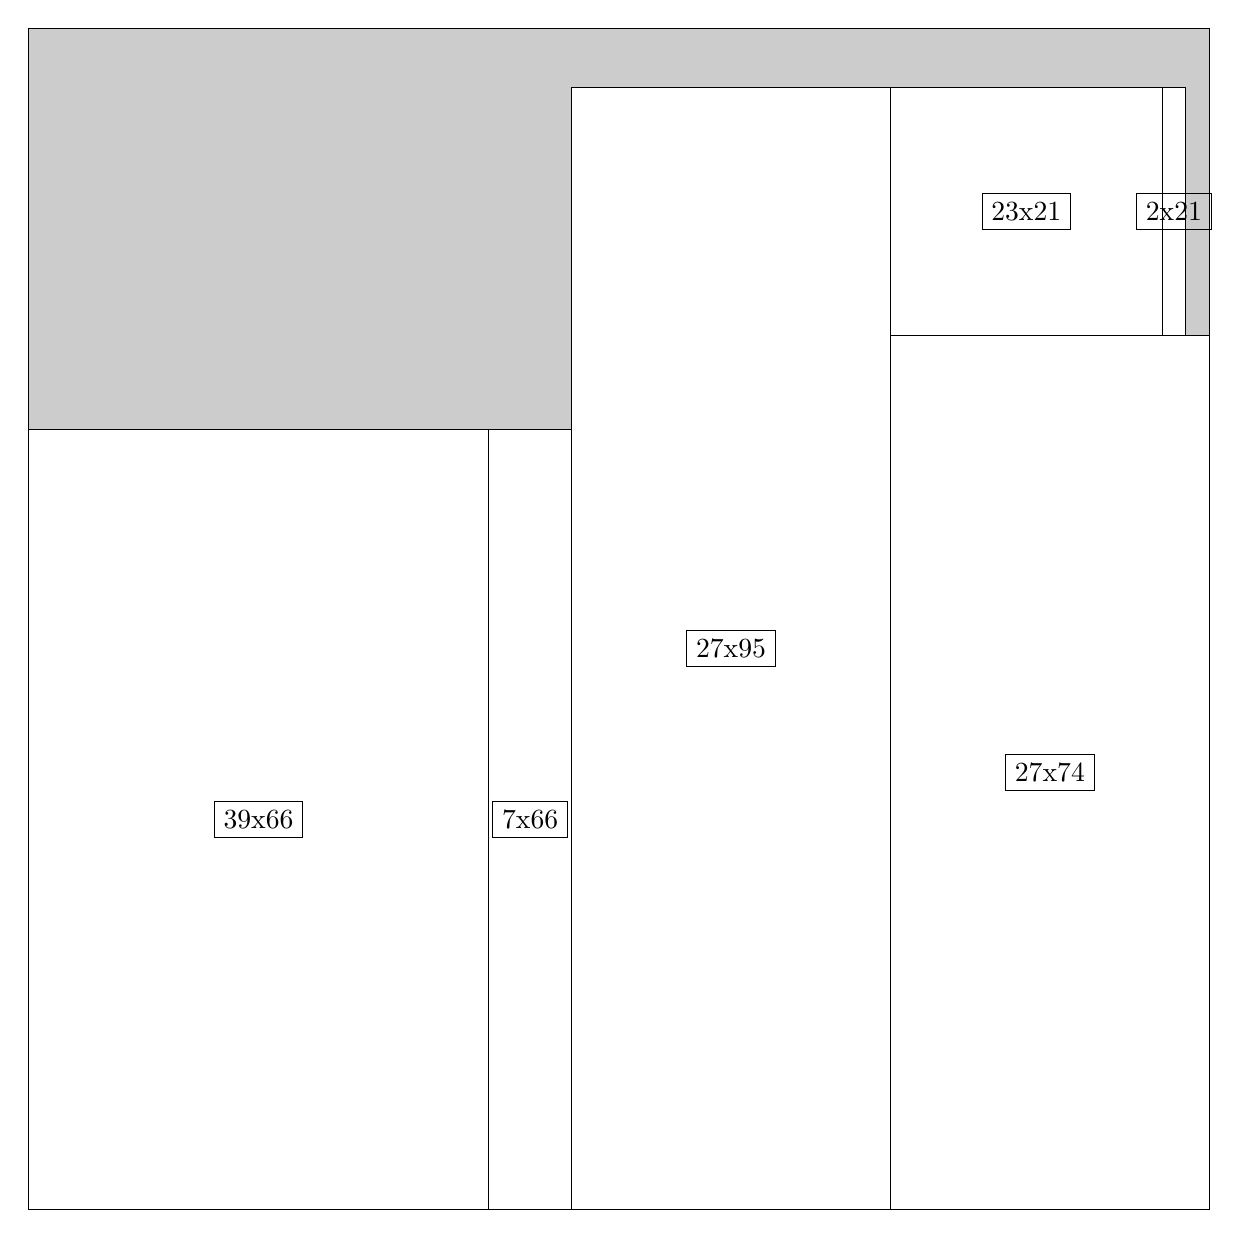
\begin{tikzpicture}[shorten >=1pt,scale=1.0,every node/.style={scale=1.0},->]
\tikzstyle{vertex}=[circle,fill=black!25,minimum size=14pt,inner sep=0pt]
\filldraw[fill=gray!40!white, draw=black] (0,0) rectangle (15.0,15.0);
\foreach \name/\x/\y/\w/\h in {39x66/0.0/0.0/5.85/9.9,27x95/6.8999999999999995/0.0/4.05/14.25,27x74/10.95/0.0/4.05/11.1,23x21/10.95/11.1/3.4499999999999997/3.15,7x66/5.85/0.0/1.05/9.9,2x21/14.399999999999999/11.1/0.3/3.15}
\filldraw[fill=white!40!white, draw=black] (\x,\y) rectangle node[draw] (\name) {\name} ++(\w,\h);
\end{tikzpicture}


w =39 , h =66 , x =0 , y =0 , v =2574
\par
w =27 , h =95 , x =46 , y =0 , v =2565
\par
w =27 , h =74 , x =73 , y =0 , v =1998
\par
w =23 , h =21 , x =73 , y =74 , v =483
\par
w =7 , h =66 , x =39 , y =0 , v =462
\par
w =2 , h =21 , x =96 , y =74 , v =42
\par
\newpage


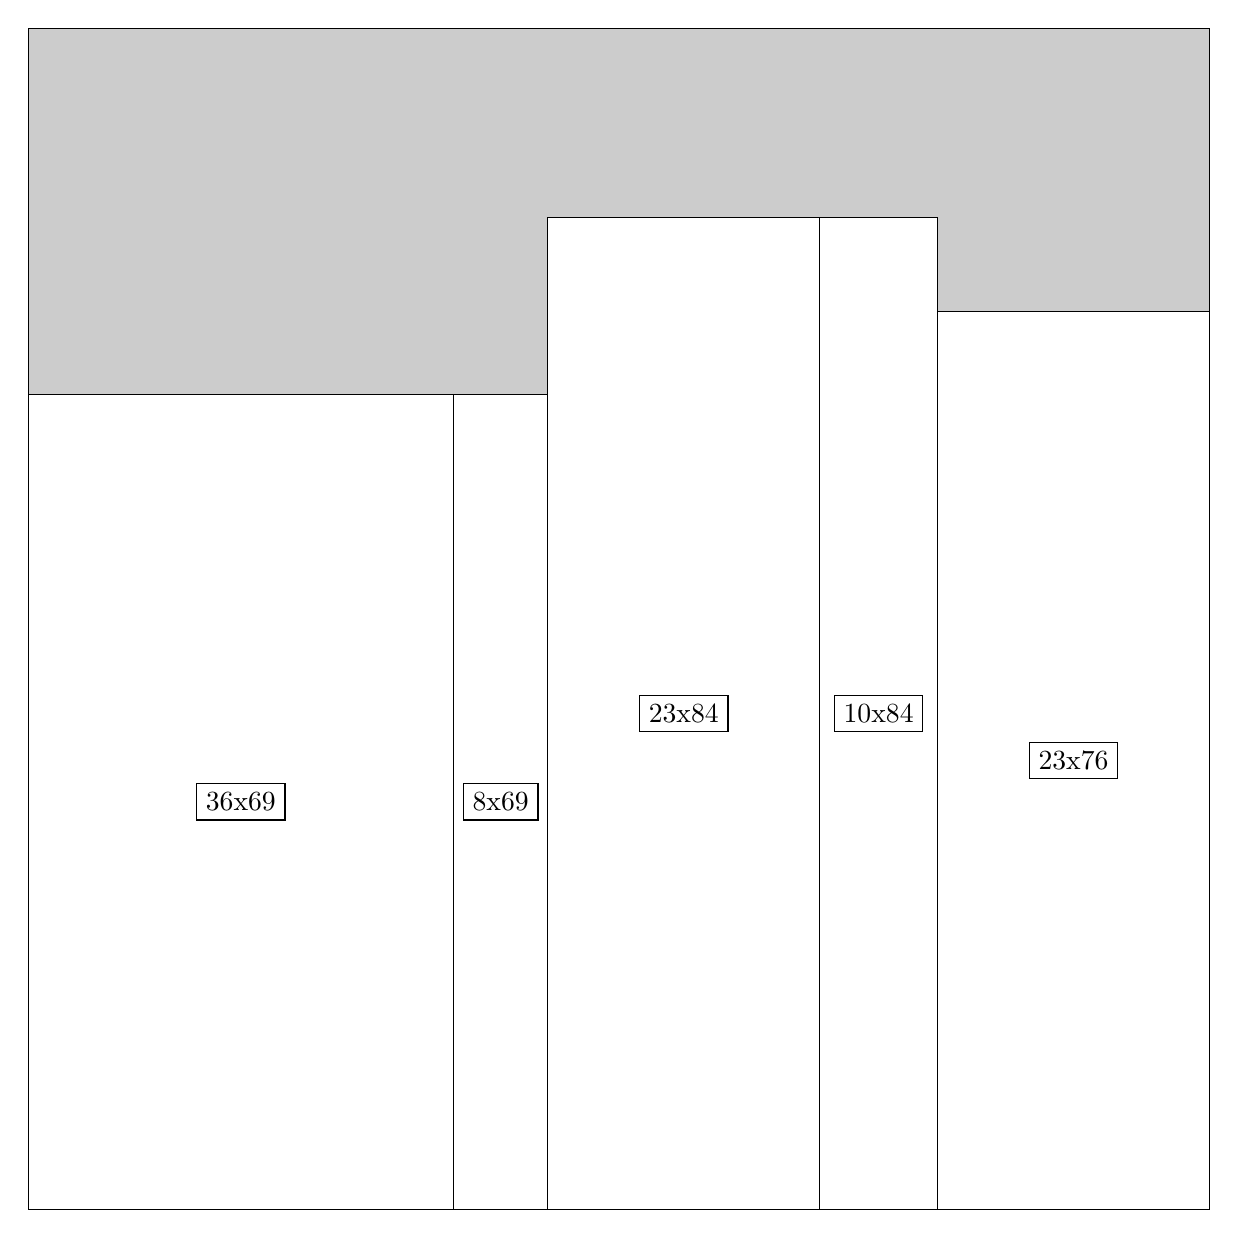
\begin{tikzpicture}[shorten >=1pt,scale=1.0,every node/.style={scale=1.0},->]
\tikzstyle{vertex}=[circle,fill=black!25,minimum size=14pt,inner sep=0pt]
\filldraw[fill=gray!40!white, draw=black] (0,0) rectangle (15.0,15.0);
\foreach \name/\x/\y/\w/\h in {36x69/0.0/0.0/5.3999999999999995/10.35,23x84/6.6/0.0/3.4499999999999997/12.6,23x76/11.549999999999999/0.0/3.4499999999999997/11.4,10x84/10.049999999999999/0.0/1.5/12.6,8x69/5.3999999999999995/0.0/1.2/10.35}
\filldraw[fill=white!40!white, draw=black] (\x,\y) rectangle node[draw] (\name) {\name} ++(\w,\h);
\end{tikzpicture}


w =36 , h =69 , x =0 , y =0 , v =2484
\par
w =23 , h =84 , x =44 , y =0 , v =1932
\par
w =23 , h =76 , x =77 , y =0 , v =1748
\par
w =10 , h =84 , x =67 , y =0 , v =840
\par
w =8 , h =69 , x =36 , y =0 , v =552
\par
\newpage


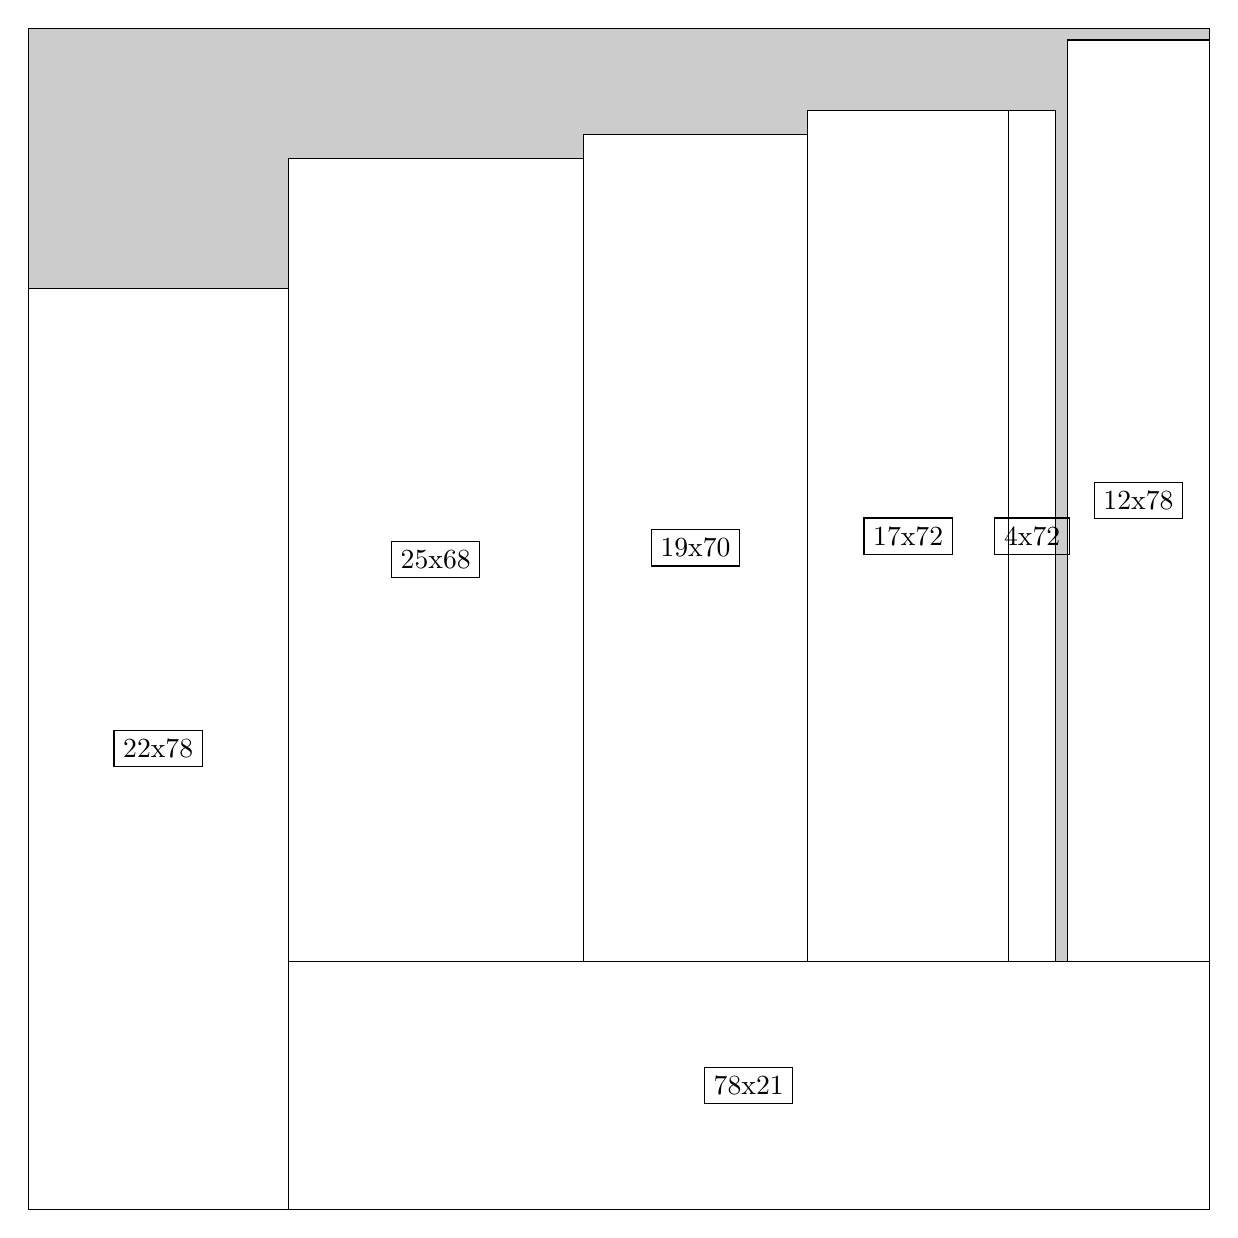
\begin{tikzpicture}[shorten >=1pt,scale=1.0,every node/.style={scale=1.0},->]
\tikzstyle{vertex}=[circle,fill=black!25,minimum size=14pt,inner sep=0pt]
\filldraw[fill=gray!40!white, draw=black] (0,0) rectangle (15.0,15.0);
\foreach \name/\x/\y/\w/\h in {22x78/0.0/0.0/3.3/11.7,25x68/3.3/3.15/3.75/10.2,78x21/3.3/0.0/11.7/3.15,19x70/7.05/3.15/2.85/10.5,17x72/9.9/3.15/2.55/10.799999999999999,12x78/13.2/3.15/1.7999999999999998/11.7,4x72/12.45/3.15/0.6/10.799999999999999}
\filldraw[fill=white!40!white, draw=black] (\x,\y) rectangle node[draw] (\name) {\name} ++(\w,\h);
\end{tikzpicture}


w =22 , h =78 , x =0 , y =0 , v =1716
\par
w =25 , h =68 , x =22 , y =21 , v =1700
\par
w =78 , h =21 , x =22 , y =0 , v =1638
\par
w =19 , h =70 , x =47 , y =21 , v =1330
\par
w =17 , h =72 , x =66 , y =21 , v =1224
\par
w =12 , h =78 , x =88 , y =21 , v =936
\par
w =4 , h =72 , x =83 , y =21 , v =288
\par
\newpage


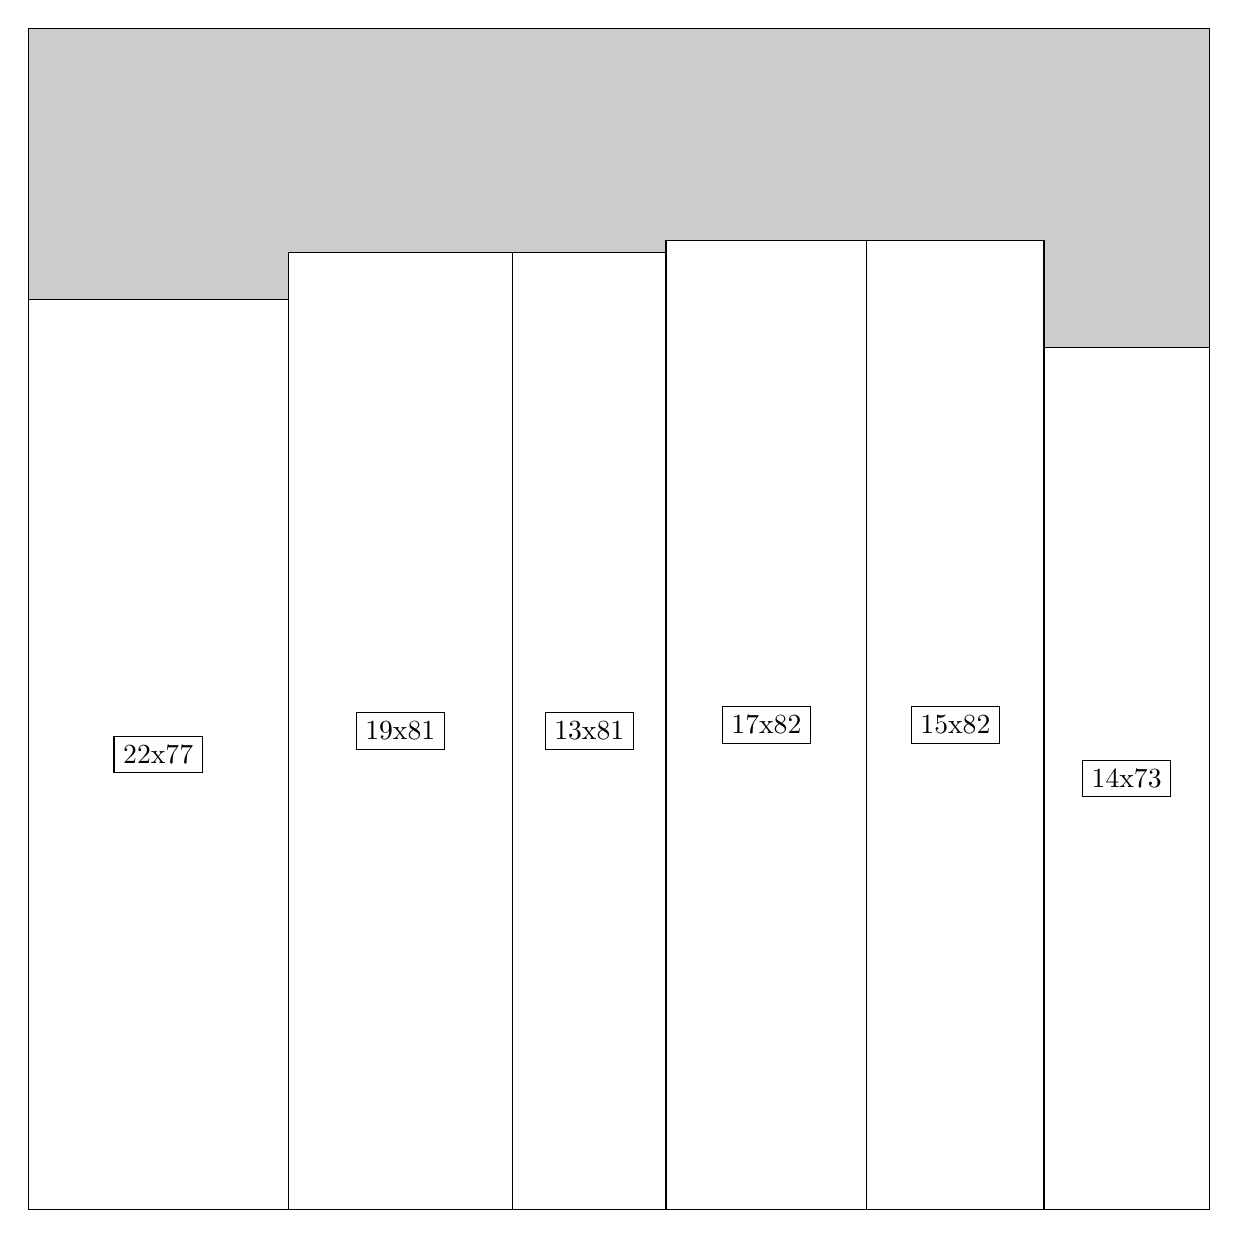
\begin{tikzpicture}[shorten >=1pt,scale=1.0,every node/.style={scale=1.0},->]
\tikzstyle{vertex}=[circle,fill=black!25,minimum size=14pt,inner sep=0pt]
\filldraw[fill=gray!40!white, draw=black] (0,0) rectangle (15.0,15.0);
\foreach \name/\x/\y/\w/\h in {22x77/0.0/0.0/3.3/11.549999999999999,19x81/3.3/0.0/2.85/12.15,17x82/8.1/0.0/2.55/12.299999999999999,15x82/10.65/0.0/2.25/12.299999999999999,13x81/6.1499999999999995/0.0/1.95/12.15,14x73/12.9/0.0/2.1/10.95}
\filldraw[fill=white!40!white, draw=black] (\x,\y) rectangle node[draw] (\name) {\name} ++(\w,\h);
\end{tikzpicture}


w =22 , h =77 , x =0 , y =0 , v =1694
\par
w =19 , h =81 , x =22 , y =0 , v =1539
\par
w =17 , h =82 , x =54 , y =0 , v =1394
\par
w =15 , h =82 , x =71 , y =0 , v =1230
\par
w =13 , h =81 , x =41 , y =0 , v =1053
\par
w =14 , h =73 , x =86 , y =0 , v =1022
\par
\newpage


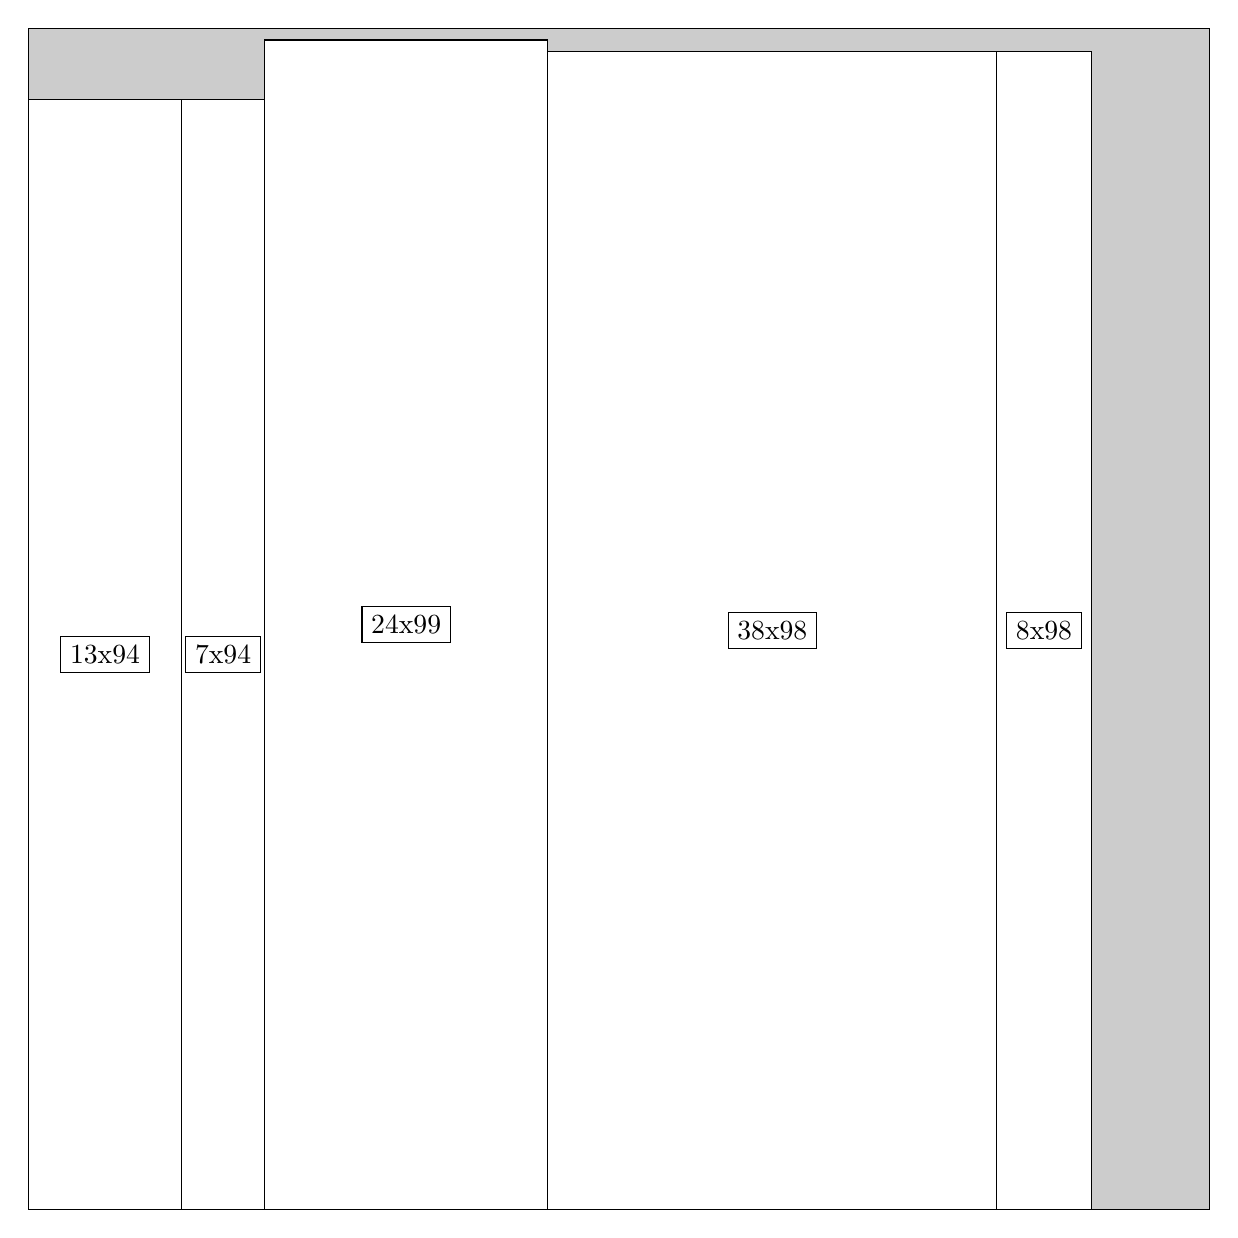
\begin{tikzpicture}[shorten >=1pt,scale=1.0,every node/.style={scale=1.0},->]
\tikzstyle{vertex}=[circle,fill=black!25,minimum size=14pt,inner sep=0pt]
\filldraw[fill=gray!40!white, draw=black] (0,0) rectangle (15.0,15.0);
\foreach \name/\x/\y/\w/\h in {38x98/6.6/0.0/5.7/14.7,24x99/3.0/0.0/3.5999999999999996/14.85,13x94/0.0/0.0/1.95/14.1,8x98/12.299999999999999/0.0/1.2/14.7,7x94/1.95/0.0/1.05/14.1}
\filldraw[fill=white!40!white, draw=black] (\x,\y) rectangle node[draw] (\name) {\name} ++(\w,\h);
\end{tikzpicture}


w =38 , h =98 , x =44 , y =0 , v =3724
\par
w =24 , h =99 , x =20 , y =0 , v =2376
\par
w =13 , h =94 , x =0 , y =0 , v =1222
\par
w =8 , h =98 , x =82 , y =0 , v =784
\par
w =7 , h =94 , x =13 , y =0 , v =658
\par
\newpage


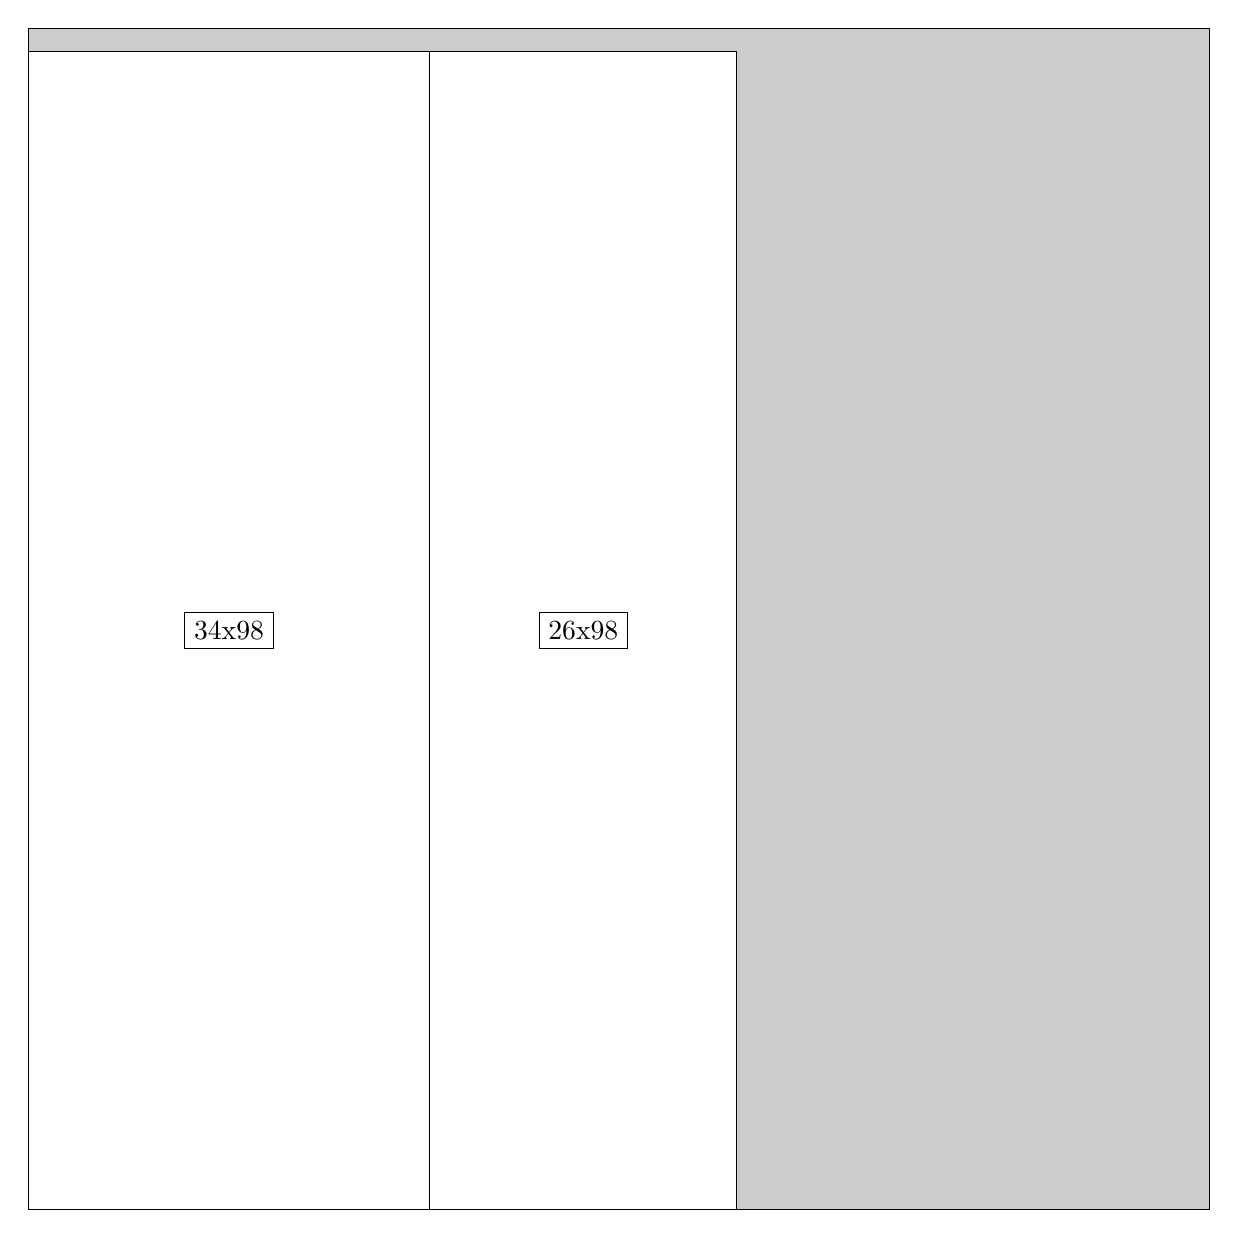
\begin{tikzpicture}[shorten >=1pt,scale=1.0,every node/.style={scale=1.0},->]
\tikzstyle{vertex}=[circle,fill=black!25,minimum size=14pt,inner sep=0pt]
\filldraw[fill=gray!40!white, draw=black] (0,0) rectangle (15.0,15.0);
\foreach \name/\x/\y/\w/\h in {34x98/0.0/0.0/5.1/14.7,26x98/5.1/0.0/3.9/14.7}
\filldraw[fill=white!40!white, draw=black] (\x,\y) rectangle node[draw] (\name) {\name} ++(\w,\h);
\end{tikzpicture}


w =34 , h =98 , x =0 , y =0 , v =3332
\par
w =26 , h =98 , x =34 , y =0 , v =2548
\par
\newpage


\end{document}